\documentclass[10pt,a4paper,ngerman, DIV=15]{scrreprt}
\usepackage{scrhack}
\usepackage{amsmath}
\usepackage{iftex}
\ifPDFTeX
	\usepackage[utf8]{inputenc}  % Deutsche Umlaute direkt eingeben
	\usepackage[T1]{fontenc}     % "Saubere" Schriften in der PDF
\else
	\ifXeTeX
		\usepackage{fontspec}
		\usepackage{unicode-math}
		\fontspec{DejaVu Serif}
		\setmainfont{DejaVu Serif} 
		\setsansfont{DejaVu Sans} 
		\setmonofont{DejaVu Sans Mono} 
		\setmathfont[math-style=TeX]{TeX Gyre DejaVu Math}
	\else
		\ifLuaTeX
			\usepackage{fontspec}
			\usepackage{luaotfload}
			\usepackage{luatextra}
%			\usepackage{lmodern}
			\usepackage{unicode-math}
			\fontspec{DejaVu Serif}
			\setmainfont{DejaVu Serif} 
			\setsansfont{DejaVu Sans} 
			\setmonofont{DejaVu Sans Mono} 
			\setmathfont[math-style=TeX]{TeX Gyre DejaVu Math}
		\fi
	\fi 				
\fi
\usepackage[ngerman]{babel}
\usepackage[ngerman]{translator}

\usepackage[babel, german=quotes]{csquotes}
\usepackage{gensymb}
\usepackage{textcomp}
\usepackage{hyperref}
\usepackage[]{varioref}
\usepackage[]{cleveref}
\usepackage{graphicx}
\usepackage{float}
\RedeclareSectionCommand[tocnumwidth=2em]{chapter}
\RedeclareSectionCommand[tocindent=3em,tocnumwidth=3.5em]{section}
\usepackage[]{todonotes}
\usepackage[toc, nopostdot, nonumberlist]{glossaries}
\makeglossaries

\usepackage{makeidx}
\makeindex

\setlength{\parindent} {0.0em}
\setlength{\parskip} {1.5ex plus0.5ex minus0.5ex}

\usepackage[backend=biber, %% Hilfsprogramm "biber" (statt "biblatex" oder "bibtex")
style=authoryear, %% Zitierstil (siehe Dokumentation)
natbib=true, %% Bereitstellen von natbib-kompatiblen Zitierkommandos
hyperref=true, %% hyperref-Paket verwenden, um Links zu erstellen
]{biblatex}
%\usepackage[backend=biber,style=alphabetic]{biblatex}
% die bib-Datei laden:
\addbibresource{Literatur.bib} %




\author{Thomas Kluth}
\title{Backbuch der Familie Kluth Stöwer}
%\setcounter{tocdepth}{3}
\setcounter{secnumdepth}{1}
\usepackage{booktabs}
\begin{document}
\maketitle
\setcounter{tocdepth}{3}
\tableofcontents

\chapter{Kuchen}
\section{Rockmannkuchen}
\subsection*{Zubereitung}
\begin{tabular}{lrr}
	Personen         &                12 &  \\
	Zubereitungszeit &               40 & Minuten \\
	Gesamtzeit       &                   & Stunden \\
%	Entnommen aus    & entnommen aus \cite{Oliver2009} &
\end{tabular} 

\subsection*{Zutaten}
\begin{tabular}{lrr}
	Preiselbeeren        &   1 &   Glas \\
	Blockschokolade      & 100 &      g \\
	Zucker               & 100 &      g \\
	gemahlene Haselnüsse & 100 &      g \\
	Backpulver           &   2 &     TL \\
	Wasser               &   3 &     TL \\
	Rum                  &   3 &   TL g \\
	Sahne                &   2 & Becher \\
	Eier                 &   4 &
\end{tabular} 

\subsection*{Zubereitung}
\begin{enumerate}
	\item Eigelb und Zucker schaumig schlagen
	\item Nüsse, Schokolade, Backpulver und Wasser zugeben. 
	\item Eischnee darunterheben
	\item 30 min. bei 170 Grad backen
	\item Tortenboden mit 3 EL Rum beträufeln, Preisselbeeren darauf.
	\item Sahne mit Sahnesteif geschlagen darüber
\end{enumerate}
  
\section{Zitronentarte mit Himbeersoße} \index{Zitronentarte}\index{Zitronen!Tarte}\index{Tarte}\index{Zitrone}
\subsection*{Zubereitung}
\begin{tabular}{lrl}
	Personen         &                12 &  \\
	Zubereitungszeit &               100 & Minuten \\
	Gesamtzeit       &                   & Stunden \\
	Entnommen aus    & entnommen aus \cite{Oliver2009} &
\end{tabular} 

\subsection*{Zutaten}
\begin{tabular}{lrl}
	Himbeeren     & 200 &     g \\
	Bio-Zitronen  &   5 & Stück \\
	Zucker        &     &  \\
	Puderzucker   & 250 &     g \\
	Vanilleschote &   1 &  \\
	Mehl          & 220 &     g \\
	Butter        & 110 &     g \\
	Sahne         & 125 &     g \\
	Eier          &   5 &
\end{tabular} 

\subsection*{Zubereitung}
\begin{enumerate}
	\item Himbeeren auftauen lassen. Zitronen heiß waschen und trocken reiben. Von 3 Zitronen die Schale fein abreiben. Mehl, 50 g Zucker und 1/4 der Zitronenschale mischen. Butter in Flöckchen, Eigelb und 2–3 EL kaltes Wasser erst mit den Knethaken des Handrührgerätes, dann mit den Händen zu einem glatten Teig verarbeiten. Zugedeckt 30 Minuten stehen lassen. Tarteform in den Kühlschrank stellen.
	\item Teig auf einer bemehlten Arbeitsfläche rund ausrollen. Eine gefettete, mit Mehl ausgestäubte Tarte-Form damit auslegen. Dabei den Rand hochziehen und andrücken. Tarteboden mit einer Gabel mehrmals einstechen. Bei Umluft 200 Grad 12 -- 15 backen. 
	\item Abgeriebene Zitronen halbieren, Saft auspressen. Vanilleschote längs aufschneiden, Mark herausschaben. Vanillemark, 200 g Puderzucker und Eier mit den Schneebesen des Handrührgerätes dick-cremig aufschlagen. Sahne steif schlagen, mit Zitronensaft und übriger Zitronenschale unter die Eier heben.
	\item Backofentemperatur auf 150 Grad herunter schalten. Vorgebackenen Teig mit Paniermehl bestreuen. Eier-Creme in die Form geben. Im  Backofen 40–50 Minuten backen, bis die Creme gestockt ist. 
	\item 3 Zitronen in sehr dünne Scheiben schneiden. 100 ml Wasser und 100 g Zucker in einem Topf aufkochen. Zitronenscheiben darin bei schwacher Hitze 2–3 Minuten glasig dünsten. Zitronenscheiben im Sud erkalten lassen.
	\item Himbeeren und 4 EL Zucker pürieren, durch ein Sieb streichen.
	\item  Tarte herausnehmen und auf einem Kuchengitter auskühlen lassen. Vor dem Servieren die Tarte mit den Zitronenscheiben belegen, mit 50 g Puderzucker bestäuben und unter dem heißen Grill des Backofens goldbraun karamellisieren. Tarte mit Himbeersoße servieren.
\end{enumerate}


\section{Flockensahne} \index{Brandteig}\index{Windbeutel!Torte}

\begin{tabular}{lrr}
	Personen         &                12 &  \\
	Zubereitungszeit &               60 & Minuten \\
	Gesamtzeit       &                3   & Stunden \\
	Entnommen aus    & Chefkoch.de &
\end{tabular} 

\subsection*{Zutaten}
\textbf{Für den Mürbeteig:}\\
\begin{tabular}{lrl}
	Mehl          & 200 &     g \\
	Zucker        &  60 &  \\
	Vanillezucker &   1 &  Pck. \\
	Butter        & 120 &     g \\
	Eier          &   1 &  \\
	Salz          &   1 & Prise \\
	Speisestärke  &  15 &     g
\end{tabular} 

\textbf{Für den Brandteig:}\\
\begin{tabular}{lrl}
	Mehl          & 250 &         g   \\
	Backpulver    &   2 &      Msp.   \\
	Vanillezucker &   2 &      Pck.   \\
	Butter        & 140 &         g   \\
	Wasser        & 500 & ml\\
	Eier &  & 6
\end{tabular} 

\textbf{Für die Füllung:}\\
\begin{tabular}{lrl}
	Sahnesteif    &    5 & Pck.Msp. \\
	Vanillezucker &    5 &     Pck. \\
	Sahne         & 1000 &       ml \\
	Preiselbeeren &    1 &     Glas \\
	Himbeeren     &      &
\end{tabular} 


\subsection*{Zubereitung}
\begin{enumerate}
	\item Aus den Zutaten für den Mürbeteig einen Teig zubereiten und ca. 1 Std. kalt stellen.
	Einen Backrahmen zusammenstecken ( ca.35x25cm ). Darin den Mürbeteig ausrollen und mit einer Gabel mehrmals einstechen. Bei 180\degree\  ca. 10-15 Min. backen.
	
	\item Für den Brandteig das Wasser mit der Butter und dem Vanillezucker aufkochen, das Mehl mit dem Backpulver dazugeben und so lange rühren, bis sich ein Teigklumpen gebildet hat. Etwas abkühlen lassen.\\
	Danach jedes Ei einzeln unterrühren, bis sich eine zähe "Pampe" gebildet hat.
	
	\item Zwei Backbleche mit Backpapier auslegen und den Teig auf die beiden Bleche verteilen und dünn verstreichen. Die Brandteigböden sollen größer werden als der Mürbeteigboden, da man später noch etwas zum obenauf streuen benötigt. Die Böden nacheinander bei 200\degree\  ca. 35 min backen. Den Backofen zwischendurch nicht öffnen, sonst fällt der Teig zusammen.\\
	Mit Hilfe des Backrahmens jeden Brandteigboden in der Größe des Mürbeteigbodens ausstechen und die Reste des Brandteiges aufheben.
	
	\item Den Mürbeteigboden in den Backrahmen legen und mit Konfitüre bestreichen. Ich nehme immer pürierte Preiselbeeren aus dem Glas. Dann eine Brandteigplatte auflegen. Mit einem Teelöffel kleine Häufchen Preiselbeeren auf dem Boden verteilen.
	
	\item Die Sahne mit dem Sahnesteif und dem Vanillezucker steif schlagen. Die Hälfte davon auf den Boden geben und verteilen. Dann den 2. Brandteigboden auflegen. Wieder Preiselbeerhäufchen verteilen und die restliche Sahne darauf verteilen und glatt streichen. Die Reste der beiden Brandteigböden fein auseinander zupfen und wie Flocken auf dem Kuchen verteilen.
	
	\item Den Kuchen zum Schluss mit Puderzucker bestäuben.
	\item Den Kuchen mindestens 2 Std. kalt stellen. Ich habe diesen Kuchen auch schon einen Tag vorher zubereitet. Das tut dem Geschmack keinen Abbruch. 
\end{enumerate}

\section{Windbeutel} \index{Brandteig}\index{Windbeuteltorte}

\subsection*{Zutaten}

\begin{itemize}
	\item 50 g Butter
	\item 1/2 TL Salz
	\item 	150 g Mehl (Type 405)
	\item 	4 M Eier
	\item 	400 g Sahne 
	\item 	1-2 EL Zucker 
	\item 	2 Päckchen Bourbon-Vanillezucker 
	\item 	Backpapier für das Blech 
	\item 	Puderzucker zum Bestreuen
\end{itemize}

\subsection*{Zubereitung}

Für die Brandmasse die Butter in Stückchen mit 250 ml Wasser und Salz in einem Topf aufkochen. Sobald sie geschmolzen ist, das Mehl auf einmal hinein schütten. Mit einem Kochlöffel kräftig rühren, bis sich ein Kloß gebildet hat und am Topfboden ein weißer Belag zu sehen ist. Den Teig in eine Rührschüssel geben. Ein Ei nach dem anderen gründlich mit den Knethaken des Handrührgeräts unter den warmen Teig rühren. 

Den Backofen auf 200° (Umluft 180°) vorheizen. Mit großem Abstand zwölf Rosetten auf ein Blech mit Backpapier mittels zweier Löffel setzen. Das Blech in den Ofen (Mitte) schieben, ein mit Wasser gefülltes zweites Backblech auf der untersten Schiene und rasch die Backofentür schließen. Die Windbeutel in 20-25 Min. goldbraun backen (dabei die Ofentür nicht öffnen!). 

Herausnehmen, von jedem einen Deckel abschneiden und auf einem Kuchengitter auskühlen lassen.

Für die Füllung die Sahne mit Zucker und Vanillezucker steif schlagen und in einen Spritzbeutel mit großer Sterntülle füllen. Die unteren Hälften der Windbeutel mit der Vanillesahne füllen, die Deckel aufsetzen und das Gebäck mit Puderzucker bestreuen.



\section{Käsekuchen mit Mohn} \index{Mürbeteig}\index{Kuchen!Käse}\index{Mohn}
\subsection*{Zutaten}
Für 26\,cm / 28\,cm Springform 

\subsubsection*{Für die Mohnmasse}
\begin{tabular}{lrl}
    Milch          & 250 & ml \\
    Butter         &  60 &  g \\
    Zucker         &  60 &  g \\
    Mohn           & 250 &  g \\
    Zitronenabrieb &   1 & TL
\end{tabular} 
\subsubsection*{Für den Mürbeteig}
\begin{tabular}{lrl}
    Mehl 550     &  220 /260 &             g \\
    Ei           &         1 & mittel / groß \\
    Butter, kalt & 110 / 130 &             g \\
    Zucker       &   70 / 80 &            EL \\
    Backpulver   &       0,5 &            TL
\end{tabular} 

\subsubsection*{Für die Quarkcreme}
\begin{tabular}{lrl}
    weiche Butter  &   80 / 95 &             g \\
    Zucker         & 100 / 115 &             g \\
    Eier           &         2 & mittel / groß \\
    Quark          &  500 /580 &             g \\
    Schmand        & 200  /230 &             g \\
    Zitronenabrieb &         2 &            TL \\
    Zitronensaft   &         2 &            EL \\
    Speisestärke   &    25 /30 &             g
\end{tabular} 

\begin{enumerate}
    \item Milch, Butter, Zucker und Zitronenabrieb in einem kleinen Topf aufkochen. Mohn einrühren und 1-2 Minuten auf niedriger
    Stufe einköcheln lassen. Vom Herd nehmen. Deckel aufsetzen und quellen lassen, bis die Mohnmasse gebraucht wird.
    \item Für den Teig alle Zutaten miteinander verkneten. Die Springform leicht fetten. Teig ausrollen, sodass man Boden und ca. 3
    cm hoher Rand formen kann. Teig in die Form legen und kühl stellen.
    \item Backofen auf 180 Grad Ober- und Unterhitze vorheizen. Weiche Butter mit Zucker schaumig schlagen, Eier einzeln
    unterrühren. Quark, Schmand, Speisestärke, Zitronensaft und -abrieb ebenfalls unterrühren.
    \item Die Mohnmasse auf den Teig geben und glatt streichen. Quarkcreme darüber verteilen. Kuchen ca. 45 Minuten backen. Am
    besten im ausgeschalteten Ofen abkühlen lassen.
\end{enumerate}


\section{Pflaumenkuchen mit Mandelstreusel} \index{Hefeteig}\index{Pflaumen}\index{Zwetchgen}
\subsection*{Zutaten}

\begin{tabular}{lrr}
    Mehl           & 175 &  g \\
    frische Hefe   &  10 &  g \\
    lauwarme Milch &  80 & ml \\
    Butter         &  25 &  g \\
    Ei             &   1 &    \\
    Zucker         &   2 & EL \\
    Zwetschgen     & 500 &  g
\end{tabular} 

Für die Streusel:\\
\begin{tabular}{lrr}
    flüssige Butter &  75 &     g \\
    Mehl            & 120 &     g \\
    Zucker          &  60 &     g \\
    Salz            &   1 & Prise \\
    Zimt            &   1 & Prise
\end{tabular} 

\subsection*{Zubereitung}
\begin{enumerate}
	\item Das Mehl in eine Schüssel geben und eine Mulde in die Mitte drücken, die Hefe dort hinein bröseln und mit der lauwarmen Milch und ein wenig Mehl vom Rand der Mulde zu einem Vorteig verrühren. Das Ganze dann zugedeckt an einem schönen warmen Ort 15 Minuten gehen lassen.
	\item Die Butter schmelzen und zusammen mit dem Ei und dem Zucker zu dem Vorteig geben und alles mit einander verkneten. Den Teig nun weitere 15 Minuten zugedeckt gehen lassen.
	\item Derweil die Zwetschgen waschen, entsteinen und in Viertel schneiden.
	\item Sobald der Teig fertig aufgegangen ist, ihn auf einer bemehlten Oberfläche ausrollen und in eine vorbereitete 26 cm Springform geben. Mit etwas Teig einen Rand ausformen und mit einer Gabel mehrfach in den Boden pieksen. Anschließend die Zwetschgenviertel dicht aneinander gepackt auf dem Hefeteig verteilen.
	\item Alle trockenen Zutaten (Mehl, Zucker, Mandeln, Salz und Zimt) in eine Schüssel geben und die flüssige Butter darüber gießen. Nun alles kräftig mit einander verkneten, bis ein krümeliger Teig entsteht.
	\item Die Streusel auf die Zwetschgen geben, so viele wie gewollt und den Kuchen bei 180°C für etwa 40 Minuten backen, bis die Streusel goldbraun sind.
\end{enumerate}

Für ein Blech zwei große Eier und ansonsten die dreifache Menge von allem.

\section{Johannisbeer Quark \textmd{(siehe \cite[172]{OetkerBackenMachtFreude1992})}}\index{Johannisbeeren}

\section{Aprikosen Tarte} \index{Aprikosen}\index{Tarte!Aprikose}

\chapter{Plätzchen}

\section[Cantuccini]{Cantuccini \textmd{(siehe \cite{ChefkochCantuccini})}}
Mandelplätzchen aus der Toscana/Umbrien
\subsection*{Zutaten}

\begin {tabular}{r l}
    350 g & Mandeln \\
    500 g & Mehl \\
    360 g & Zucker \\
    2 TL & Backpulver \\
    4 Pkt. & Vanillezucker \\
    1 Flasche & Bittermandelaroma \\
    2 Priesen & Salz \\
    50 g & Butter, zimmerwarme \\
    4 & Eier
\end{tabular}
\subsection*{Zubereitung}
\begin{enumerate}
    \item  Alle Zutaten (bis auf die Mandeln) zu einem Knetteig verarbeiten: ein klebriger Knetteig!
    \item  Die Mandeln unterkneten. Den Teig mit etwas Mehl zu einer Kugel formen und 30 Minuten kalt stellen.
    \item  Den Teig in 12 Teile schneiden. Aus jedem Teil eine 25 cm lange Rolle formen. Das Backblech mit Backtrennpapier auslegen. Die Rollen im
    Abstand von 8 cm voneinander auflegen.
    \item  Im vorgeheizten Backofen bei 200 °C Ober-/Unterhitze 15 Minuten vorbacken, kalt werden lassen und dann schräg in 1 cm dicke
    Scheiben schneiden.
    \item  Plätzchen mit einer Schnittfläche auf das Backblech legen und noch einmal im Backofen bei gleicher Temperatur 10 Minuten rösten. Die Cantuccini müssen zum Schluss
    goldbraun sein.
    \item  Die Plätzchen auskühlen lassen und in einer geschlossenen Blechdose aufbewahren, sonst werden sie weich. 
\end{enumerate}


\chapter{Pizza, Quiche  \& Co}

\section{Pizza-Teig}\label{sec:Pizza-Teig}\index{Pizza-Teig}
\subsection*{Zeitplan}
\begin{tabular}{ r @{ Uhr \phantom{bla} } l}
    \toprule
    \multicolumn{1}{c @{\phantom{ bla }}}{Zeit} & \multicolumn{1}{@{}l}{Aktion}           \\ \midrule
    00:00                                       & \Gls{Hauptteig}                         \\ \midrule
    \multicolumn{2}{c @{\phantom{ bla }}}{Schnelle Variante}                \\
    00:20                                       & \Gls{Stockgare}                         \\
    02:00                                       & \Gls{Formen}                            \\
    02:10                                       & \Gls{Stueckgare}                        \\
    03:10                                       & \Gls{Backen}                            \\ \midrule
    \multicolumn{2}{c @{\phantom{ bla }}}{Kalte Variante}                 \\
    00:20                                       & \Gls{Stockgare} 1                       \\
    00:50                                       & \Gls{DehnenUndFalten} + \Gls{Stockgare} 2 \\
    05:00 / 09:00                               & \Gls{Formen}                            \\
    05:10 / 09:10                               & \Gls{Stueckgare}                        \\
    06:10 / 10:10                               & \Gls{Backen}                            \\ \bottomrule
\end{tabular}

\subsection*{Zutaten für 6 Pizzen}
\begin{tabular}{r l}
    10\;g & frische Hefe  \\
    600\;ml & kaltes Wasser \\
    1\;kg & Mehl          \\
    8\;g & Salz
\end{tabular} 


\subsection*{Zubereitung}

Es gibt die schnelle und die \glqq langsame\grqq\ Variante
\begin{enumerate}
    \item [\Gls{Hauptteig}] Hefe in 600 ml kaltes Wasser bröseln und 5 Minuten gut durch rühren.\\
    Mehl mit Salz zum Hefewasser geben und zu einem Teigkloß verarbeiten. Teig 10 Minuten mit langsam und dann ca. 5 Minuten schnellermit knetenden Händen (Maschine funktioniert nicht wirklich) auf einer leicht bemehlten Oberfläche 10-15 Minuten geschmeidig kneten.
    \item  \textbf{Langsame Variante}
    \begin{itemize}
        \item Teig in eine große geölte Plastikdose geben und nach 30 Minuten dehnen und falten. Danach bis zu 8 Stunden in den Kühlschrank stellen. 
        \item 2 Stunden vor dem Backen den Teig auf die Arbeitsfläche gleiten lassen, falten und dehnen, wieder in die Dose geben.
        \item Abgedeckt nochmals 30 Minuten bei Zimmertemperatur gehen lassen. 
    \end{itemize}
    \item \textbf{Schnelle Variante}
    \begin{itemize}
        \item Teig Schüssel geben und luftdicht abschließen.
        \item Abgedeckt 1:30 Minuten bei Zimmertemperatur gehen lassen. 
    \end{itemize}
    \item [\Gls{Formen}] Teig auf der leicht bemehlten Arbeitsfläche zu einer Rolle formen, dabei nicht zu viel kneten.
    Rolle in 6 gleich große , ca. 250 g schwere Stücke teilen.
    Teigstücke zu Kugeln formen, mit ca. 10 cm Abstand in eine leicht bemehlte Form legen. 
    \item [\Gls{Stueckgare}] Mit Mehl bestäuben und abgedeckt bei Zimmertemperatur eine Stunde gehen lassen.
    \item [\Gls{Backen}] Teigkugeln jeweils mit den Händen auf der bemehlten Arbeitsfläche von innen nach außen zu dünnen runden oder ovalen Fladen drücken, den dabei entstehenden Rand nicht flachdrücken. \\
    Fladen jeweils auf ein Stück Backpapier geben, belegen und backen.
\end{enumerate}
%
\section[Pizzateig mit wenig Hefe und LM]{Pizzateig mit wenig Hefe und Lievito Madre \textmd{(siehe \cite{sonjaPizza}})}\label{sec:Pizza-Teig-2}\index{Pizza-Teig}
\subsection*{Zeitplan}
\begin{tabular}{ r @{ Uhr \phantom{bla} } l}
    \toprule
    \multicolumn{1}{c @{\phantom{ bla }}}{Zeit} & \multicolumn{1}{@{}l}{Aktion}           \\ \midrule
    00:00                                       & \Gls{Autolyse}                         \\ 
    00:20                                       & \Gls{Hauptteig}                         \\ 
    00:40                                       & \Gls{Stockgare}                         \\
    01:40                                       & \Gls{Formen}                            \\
    01:50                                      & \Gls{Stueckgare}                        \\
    13:50  / 73:50                                     & \Gls{Akklimatisieren}                            \\ 
    15:00  / 75:00                                       &  \Gls{Backen}                            \\ \bottomrule
\end{tabular}

\subsection*{Zutaten für 4 Pizzen}
\begin{tabular}{r l}
    60\;g & Lievito Madre aufgefrischt  \\
    2\;g & frische Hefe  \\
    380\;ml & kaltes Wasser \\
    600\;g & Tipo 00          \\
    12\;g & Salz
\end{tabular} 


\subsection*{Zubereitung}

Es gibt die schnelle und die \glqq langsame\grqq\ Variante
\begin{enumerate}
    \item [\Gls{Autolyse}] Wasser und Mehl kurz vermischen. Abgedeckt für 20 Minuten quellen lassen.
    
    \item [\Gls{Hauptteig}] Lievito Madre und Hefe hinzufügen, für 8−10 Minuten langsam kneten. Danach Salz hinzugeben. Für weitere 4−8 Minuten schnell auskneten.
    \item [\Gls{Stockgare}] Den Teig in eine geölte Teigwanne geben und für 60 Minuten bei Raumtemperatur (22−22 °C) reifen lassen.
    Dabei nach 30 Minuten einmal dehnen und falten.
    \item [\Gls{Formen}]  Anschließend den Teig in 4 gleich große Teiglinge teilen. Jeweils zu einer 4 Kugeln rund wirken.
    \item [\Gls{Stueckgare}]  Die Kugeln leicht einölen und zurück in die Teigwanne setzen. Für insgesamt 12−72 Stunden in einer leicht geölten Schüssel oder Teigwanne in den Kühlschrank (4−5 °C) geben.
    \item [\Gls{Akklimatisieren}] Rechtzeitig den Backofen so heiß wie möglich vorheizen, möglichst auf 280−300 °C Ober-/Unterhitze,\\
    Den Teig nach der kalten Gare mindestens 30−60 Minuten akklimatisieren lassen.
    \item[Belegen] 
    Die Teigballen aus der Teigwanne entnehmen und auf die gut mit Hartweizenmehl bemehlte Arbeitsfläche geben.\\
    Vorsichtig ringsherum mit den Fingerspitzen einen Rand abdrücken.
    Anschließend behutsam von innen nach außen etwas auseinanderziehen und -dehnen. (Nicht ausrollen!!!)\\
    Die Pizzaiola (sparsam) auf dem Teig verteilen und mit Mozzarella belegen.\\
    Danach mit den weiteren Zutaten nach Wahl belegen.\\
    Nach Belieben zusätzlich mit etwas Olivenöl beträufeln und eventuell mit getrocknetem Oregano bestreuen. (Frische Kräuter erst nach dem Backen auf die Pizza geben.)
    \item [\Gls{Backen}] Bei 280−300 °C jeweils für ca. 6−10 Minuten backen. 
\end{enumerate}
%

\section{Pizzaiola}
\subsection*{Zutaten für 4 Pizzen}

\begin{tabular}{r l}
         400\;g & Tomaten aus der Dose                                     \\
          30\;g & getrocknete Tomaten in Öl eingelegte getrocknete Tomaten \\
          10\;g & Olivenöl                                                 \\
          1\;TL & getrockneter Oregano                                     \\
            1\; & Knoblauchzehe optional                                   \\
    nach Bedarf & Salz
\end{tabular} 
\subsection*{Zubereitung}
Alle Zutaten für die Pizzaiola je nach Belieben grob bis fein pürieren.


\section{Quiche} \label{sec:Quiche}\index{Quiche}
\subsection*{Allgemeines}
\begin{tabular}{lrl}
    Personen         &   4 &  \\
    Zubereitungszeit &   40 & Minuten \\
    Woher & & ?%\cite[vgl.][]{OttoLenghiJerusalem}
\end{tabular} 

\subsection*{Zutaten}
\begin{tabular}{lrl}
    \multicolumn{3}{l}{\textbf{Teig}}                      \\
    250 &          g & Mehl                                \\
    150 &         ml & Butter                              \\
    1   &            & Eigelb                              \\
    4   &         EL & kaltes Wasser                       \\
        &            & Salz                                \\
    \multicolumn{3}{l}{\textbf{Dinkel Teig}}               \\
    210 &          g & Dinkelmehl 630                      \\
    50  &          g & Weizen 405                          \\
    125 &         ml & Butter                              \\
    1   &            & Ei                                  \\
    3   &         EL & kaltes Wasser                       \\
    30  & G Parmesan &                                     \\
        &            & Salz                                \\
    \multicolumn{3}{l}{\textbf{Sauerteig}}                 \\
    200 &          g & Weizen 405                          \\
    75  &          g & Lievieto Madre 405                  \\
    125 &         ml & Butter                              \\
    1   &            & Ei                                  \\
    3   &         EL & kaltes Wasser                       \\
    25  & G Parmesan &                                     \\
        &            & Salz                                \\
    \multicolumn{3}{l}{\textbf{Füllung}}                   \\
    300 &          g & Käse (käftig)                       \\
    150 &          g & Schinkespeck (ggf. ersetzen)        \\
    1   &            & Zwiebel                             \\
    4   &          g & Eier + 1 Eiweiß                     \\
    200 &          g & Schmand oder saure Sahne            \\
    1   &       Bund & Schnittlauch                        \\
        &            & Salz, Pfeffer, 1 TL Paprika edelsüß
\end{tabular} 
\subsection*{Zubereitung}
\begin{enumerate}
    \item Alle Zutaten für den Teig bei niedriger Stufe mit Knethaken gut vermengen. 
    \item Den fertigen Teig mindestens 30 Minuten in den Kühlschrank stellen.
    \item Eine Quiche Form einfetten. Den Teig in die Form geben, mit einer Gabel einstechen und bei 200 Grad ca. 20 Minuten backen.
    \item Die Zutaten für die Füllung vermengen und auf den Teig geben und bei 200 Grad 30 Minuten garen. In der Mitte mit einer Gabel prüfen, ob die Füllung gestockt hat. Wenn nicht weiter backen, dann aber abdecken.
\end{enumerate}

\section{Crespelle} \label{sec:Crespelle}\index{Crespelle}
\subsection*{Allgemeines}
%\begin{tabular}{lrl}
%    Personen         &   4 &  \\
%    Zubereitungszeit &   40 & Minuten \\
%    Woher & & ?%\cite[vgl.][]{OttoLenghiJerusalem}
%\end{tabular} 

\subsection*{Zutaten}
\begin{tabular}{lrl}
    120 &          g & Tipo 00                      \\
    250 &         ml & Milch                             \\
    2   &            & Eier                                  \\
    &            & Salz, Pfeffer                                \\
\end{tabular} 
%\subsection*{Zubereitung}
%\begin{enumerate}
%    \item Alle Zutaten für den Teig bei niedriger Stufe mit Knethaken gut vermengen. 
%    \item Den fertigen Teig mindestens 30 Minuten in den Kühlschrank stellen.
%    \item Eine Quiche Form einfetten. Den Teig in die Form geben, mit einer Gabel einstechen und bei 200 Grad ca. 20 Minuten backen.
%    \item Die Zutaten für die Füllung vermengen und auf den Teig geben und bei 200 Grad 30 Minuten garen. In der Mitte mit einer Gabel prüfen, ob die Füllung gestockt hat. Wenn nicht weiter backen, dann aber abdecken.
%\end{enumerate}


\chapter{Backferment Brot}
\todo{Erstellung Grundansatz}
\section{Dinkelvollkornbrot} \index{Brot!Dinkel}\index{Vollkorn!Brot}\index{Backferment!Brot}
\subsection*{Allgemeines}

\begin{tabular}{lrl}
    Gesamtzeit          & 16 --  24 & Stunden           \\
    Vorteig erstellen   &        10 & Minuten           \\
    Vorteig             &  12 -- 16 & Stunden           \\
    Brühstück           &        10 & Minuten           \\
    Gehzeit             &        30 & Minuten           \\
    Hauptteig erstellen &        10 & Minuten           \\
    1. Gehzeit          &        50 & Minuten           \\
    2. Gehzeit          &  30 -- 50 & Minuten           \\
    Backzeit            &         1 & Stunde \\ 
    && \cite[Seite 159 ]{Pokorny2016}
\end{tabular} 

\subsection*{Zutaten}

\subsubsection*{Vorteig}
\begin{tabular}{lrr}
    Dinkelvollkornmehl                  & 150 &  g \\
    lauwarmes Wasser (ca. 40 $^\circ$C) & 150 & ml \\
    Grundansatz                         &  10 &  g \\
    Backferment                         &   3 &  g
\end{tabular} 

Grundansatz mit Backferment in etwas Wasser auflösen, restliches Wasser zugeben und mit dem Vollkornmehl gründlich vermengen. Bedeckt bei ca. 24 $^circ $C mindestens 12 Stunden stehen lassen. 

\subsubsection*{Brühstück}
\begin{tabular}{lrr}
    Dinkelvollkornmehl                  & 100 (150) &  g \\
    kochendes Wasser  & 180 (280) & ml \\
\end{tabular} 

Mehl mit dem Wasser (genau abmessen) über brühen. Gut durchkneten. Das Brühstück soll ziemlich fest, aber nicht hart sein. Falls nötig nochmal etwas kochendes Wasser einarbeiten. Bedeckt ca. 30 Minuten ausquellen lassen.  

\subsubsection*{Hauptteig}
\begin{tabular}{lrr}
    Dinkelvollkornmehl & 250 &  g \\
    sehr warmes Wasser (ca. 45 $^\circ$C) & 150 (50) & ml \\
    Hefe   & 2-3          &   g \\
    Salz        & 10 & g \\
\end{tabular} 

\subsection*{Zubereitung}

\begin{enumerate}
    \item Den Vorteig mit dem Brühstück homogen vermengen.
    \item Zum Vorteig das gesalzene Vollkornmehl hinzugegeben und vermengen. Hefe in Wasser auflösen und nach und nach Wasser hinzugeben. Der Teig soll mittelfest sein. Zur Not etwas warmes Wasser oder Mehl hinzugeben. 
    \item Bedeckt 40 Minuten stehen lassen. Durchkneten, nach Belieben Körner (Sonnenblumen schmeckt gut, ca. 100g) hinzugeben und in warme gefettete Backformen  (oder Garkörbchen) legen.
    \item Bedeckt weitere 40 Minuten stehen lassen. Backofen vorheizen ($ 220\;^{circ} $C, Umluft $ 200\;^{circ} $C) und Wasserschüssel einstellen. Teigstücke an der Oberfläche befeuchten und ca. eine Stunde backen.    
\end{enumerate}  

\section{Weizen-Roggen-Vollkorn} \index{Brot!Weizen-Roggen}\index{Brot!Roggen}\index{Brot!Weizen}\index{Vollkorn!Brot}\index{Backferment!Brot}
\subsection*{Allgemeines}
\begin{tabular}{lrl}
    Gesamtzeit          & 16 --  24 & Stunden                       \\
    Vorteig erstellen   &        10 & Minuten                       \\
    Vorteig             &  12 -- 16 & Stunden                       \\
    Hauptteig erstellen &        10 & Minuten                       \\
    1. Gehzeit          &        50 & Minuten                       \\
    2. Gehzeit          &  30 -- 50 & Minuten                       \\
    Backzeit            &         1 & Stunden                       \\
    &           & \cite[Seite 66 ]{Pokorny2016}
\end{tabular} 
\subsection*{Zutaten}

\subsubsection*{Vorteig}
\begin{tabular}{lrr}
    Weizenvollkornmehl                  & 100 &  g \\
    Roggenvollkornmehl                  & 100 &  g \\
    lauwarmes Wasser (ca. 40 $^\circ$C) & 200 & ml \\
    Grundansatz                         &  10 &  g \\
    Backferment                         &   2 &  g
\end{tabular} 

Grundansatz mit Backferment in etwas Wasser auflösen, restliches Wasser zugeben und mit dem Vollkornmehl gründlich vermengen. Bedeckt bei ca. 24 $^{\circ} $C mindestens 12 Stunden stehen lassen. 

\subsubsection*{Hauptteig}
\begin{tabular}{lrr}
    Weizenvollkornmehl & 150 &  g \\
    Roggenvollkornmehl & 150 &  g \\
    sehr warmes Wasser (ca. 45 $^\circ$C) & 175 & ml \\
    Hefe   & 2-3          &   g \\
    Salz        & 10 & g \\
\end{tabular} 

\subsection*{Zubereitung}

\begin{enumerate}
    \item Zum Vorteig die gesalzenen Vollkornmehle hinzugegeben und vermengen, Hefe in Wasser auflösen und nach und nach Wasser hinzugeben.
    \item Bedeckt 50 Minuten stehen lassen. Durchkneten, nach Belieben Körner (Sonnenblumen schmeckt gut, ca. 100~g) hinzugeben und in warme gefettete Backformen  (oder Garkörbchen) legen.
    \item Bedeckt weitere 40 Minuten stehen lassen. Backofen vorheizen ($ 220\;^{\circ} $C, Umluft $ 200\;^{\circ} $C) und Wasserschüssel einstellen. Teigestücke an der Oberfläche befeuchten und ca. eine Stunde backen.    
\end{enumerate}  

\section{Weizen-Hafer-Vollkorn} \index{Brot!Weizen-Hafer}\index{Brot!Hafer}\index{Hafer}\index{Brot!Weizen}\index{Vollkorn!Brot}\index{Backferment!Brot}
Der Hafer sorgt für ein mildes gut schmeckendes Brot. Das Ausquellen ist unbedingt erforderlich!
\subsection*{Allgemeines}
\begin{tabular}{lrl}
    Gesamtzeit          & 16 --  24 & Stunden                       \\
    Vorteig erstellen   &        10 & Minuten                       \\
    Vorteig             &  12 -- 16 & Stunden                       \\
    Hauptteig erstellen &        10 & Minuten                       \\
    Ausquellen          &        15 & Minuten                       \\
    1. Gehzeit          &        40 & Minuten                       \\
    2. Gehzeit          &  30 -- 40 & Minuten                       \\
    Backzeit            &  50 -- 60 & Minuten                       \\
    &           & \cite[Seite 151 ]{Pokorny2016}
\end{tabular} 
\subsection*{Zutaten}

\subsubsection*{Weizen-Hafer-Mischung}
\begin{tabular}{lrr}
    Hafervollkornmehl                  & 150 &  g \\
    Weizenvollkornmehl                 & 350 &  g \\
\end{tabular} 

\subsubsection*{Vorteig}
\begin{tabular}{lrr}
    Weizen-Hafer-Mischung               & 150 &  g \\
    lauwarmes Wasser (ca. 40 $^\circ$C) & 150 & ml \\
    Grundansatz                         &  10 &  g \\
    Backferment                         &   3 &  g
\end{tabular} 

Grundansatz mit Backferment in etwas Wasser auflösen, restliches Wasser zugeben und mit dem Vollkornmehl gründlich vermengen. Bedeckt bei ca. 24 $^{\circ} $C mindestens 12 Stunden stehen lassen. 

\section{Verdoppelung \Gls{Sauerteig}}\index{Sauerteig!Zubereitung}\label{sec:Sauerteig}
Mein Sauerteig ist ein umgezogener Lievito Madre.  

\begin{enumerate}
    \item 100\;g Anstellgut werden mit 50\; g Roggenvollkornmehl und 50\;g Roggen 1150 gemischt (nicht lange kneten). 
    \item Dann bei ca. 29 -- 31 Grad 3-4 reifen lassen.
    \item Jetzt die Hälfte des Sauerteigs aufheben (Kühlschrank) für das nächste mal Backen und mit der anderen Hälfte ihr Brot backen.
    \item Braucht man mehr Brot, so kann man den Vorgang mehrmals wiederholen.
\end{enumerate}

\chapter{Sauerteig}

\section{Verdoppelung \Gls{LievitoMadre}: Hartie}\index{Lievito Madre!Zubereitung}\label{sec:Lievito Madre}

\begin{enumerate}
    \item 100\;g Anstellgut wird 50\;g Wasser gemischt und dann ca. 10 Minuten ruhen lassen.  
    \item 50 g Semola und 50 g Tipo 0 zugegeben und gut durchkneten.
    \item Dann bei ca. 29 -- 31 Grad 3-5 Stunden reifen lassen.
    \item Braucht man mehr Lievito Madre, so kann man den Vorgang mehrmals wiederholen.
\end{enumerate}

\section{Sauerteig Roggenbrot} \index{Brot!Roggen}\index{Brot!Sauerteig}\index{Sauerteig}
\subsection*{Allgemeines}
\begin{tabular}{lrl}
	Gesamtzeit          & 17 --  24 & Stunden                        \\
	Vorteig erstellen   &        10 & Minuten                        \\
	Vorteig             &  12 -- 16 & Stunden                        \\
	Hauptteig erstellen &        10 & Minuten                        \\
	1. Gehzeit          &         2 & Stunden                        \\
	2. Gehzeit          &         2 & Stunder                        \\
	Backzeit            &  50 -- 60 & Minuten                        \\
\end{tabular} 
\subsection*{Zutaten}
\begin{tabular}{lrr}
	Sauerteig                        & 300 &  g \\
	Roggenmehl                       & 500 &  g \\
	warmes Wasser (ca. 40 $^\circ$C) & 375 & ml \\
	Hefe                             & 2-3 &  g \\
	Salz                             &   3 & TL
\end{tabular} 


\subsection*{Zubereitung}

Für die Zubereitung von Sauerteig siehe \vref{sec:Sauerteig}.

\begin{enumerate}
	\item Den Natursauerteig in eine Schüssel geben und mit den	restlichen Zutaten zu einem	glatten Teig verarbeiten. In der Maschine nur langsam kneten.
	\item Den Teig mit Mehl bedeckt ca.2 Stunden bei Zimmertemperatur ruhen lassen.	
	\item Kurz durchkneten und in eine Brotform geben. Erneut 2 Stunden Ruhe.
	\item Backofen vorheizen ($ 250\;^{\circ} $C) und Wasserschüssel einstellen. Teige einschneiden, mit Wasser besprühen und bei fallender Hitze (Ende bei $180\;^{\circ}$) abbacken.
\end{enumerate}   

Man kann auch 20\% des Roggenmehls durch Weizenmehl oder Dinkelmehl ersetzen. Das ergibt ein lockeres milderes Brot.



\section[Ciabatta / Pain Paillasse]{Ciabatta / Pain Paillasse \textmd{(siehe \cite{HollensteinerCiabatta}})}  \index{Brot!Weizen}\index{Brot!Lievito Madre}\index{Ciabatta}\label{sec:brot:Ciabatta:LM}

\subsection*{Zeitplan}
\begin{tabular}{ r @{ Uhr \phantom{bla} } l}
    \toprule
    \multicolumn{1}{c @{\phantom{ bla }}}{Zeit} & \multicolumn{1}{@{}l}{Aktion}      \\ \midrule
    00:00                                & \Gls{Autolyse}                    \\
    00:15                                & \Gls{Hauptteig}                    \\
    00:35                                & \Gls{Stockgare}                    \\
    03:35                                & \Gls{Formen} \\
    03:45								 & \Gls{Stueckgare}     \\ \midrule
    \multicolumn{2}{c}{Wurzelbrot}   \\
    04:00 &   \Gls{Backen} \\ 
    04:20 & fertig\\ \midrule
    \multicolumn{2}{c}{Ciabatta}   \\
    04:30 &   \Gls{Backen} \\
    04:55 &  fertig\\ \bottomrule
\end{tabular}

\subsection*{Zutaten}

\begin{tabular}{r l}
    \toprule
    100 g & Lievito Madre TA 150 \\ \midrule
    230 g & Tipo 0               \\
    320 g & Wasser (kühl)        \\ \midrule
    230 g & Weizenmehl  550er    \\
    310 g & Wasser (kühl)        \\ \midrule
    100 g & Hartweizenmehl       \\
      8 g & Salz                 \\
      8 g & Olivenöl             \\
    3,5 g & Frischhefe           \\ \bottomrule
\end{tabular}

\subsection*{Zubereitung}
\begin{enumerate}
   \item Alle Zutaten in den Kneter geben. Mit dem Flachschlägerhaken  3 Minuten langsam rühren, bis alles zu einem Brei verrührt ist.
   \item 10 Minuten Pause.
   \item Dann auf Stufe 2-3 schalten und den Flachschlägerhaken so lange rühren lassen, bis sich der Teig komplett von der Schüssel löst. Das hat bei mir etwa 10-12 Minuten gedauert.
   \item Den Teig in eine Teigwanne geben und mindestens 2 1/2 bis 3 Stunden reifen lassen. Ggf. noch länger. Während der ersten 90 Minuten zweimal dehnen und falten. Der Teig sollte sich gut verdreifacht haben vom Volumen und stark von Gasblasen durchzogen sein.
   \item Auf die gut bemehlte Arbeitsfläche kippen und die Rückseite bemehlen. Wenn die Teigwanne rechteckig war, von den kurzen Seiten her rasch und selbstsicher zwei Stücke abstechen. Mit den bemehlten Händen greifen und auf ein Backpapier legen. Dort dann mit raschen Handbewegungen die Teigstücke 3 – 4 mal (nicht zu oft) um sich selbst drehen, sodass die Wurzelform entsteht.
   \item Wenn es Ciabatta werden sollen, lediglich abstechen und auf das Backpapier befördern. Die Wurzelbrote noch etwa 15 Minuten entspannen lassen und dann sofort backen. Lässt man sie länger reifen, verwischen die Furchen zu stark. Ciabattateiglinge können noch gut und gerne 45 Minuten Stückgare vertragen, dann werden sie innen noch luftiger.
   \item Bei 250° in den gut vorgeheizten Ofen geben und sofort schwaden. Bei konstant 250° kräftig dunkel ausbacken
\end{enumerate}
 
\section[Ciabattine] {Ciabattine \textmd{(siehe {SonjaBauer2023})}} \index{Brot!Weizen}\index{Brötchen!Lievito Madre}
\begin{tabular}{ r @{ Uhr \phantom{bla} } l}
    \toprule
    \multicolumn{1}{c @{\phantom{ bla }}}{Zeit} & \multicolumn{1}{@{}l}{Aktion}     \\ \midrule
    00:00                                       & \Gls{Autolyse}                    \\
    01:00                                       & \Gls{Hauptteig}                   \\
    01:15                                       & \Gls{Stockgare}  Raumtemperatur   \\
    05:15                                       & \Gls{Formen} und \Gls{Stueckgare} \\
    05:30                                       & \Gls{Vorheizen}                   \\
    06:00                                       & \Gls{Backen}                      \\
    06:20                                       & fertig                            \\ \bottomrule
\end{tabular}

\subsection*{Zubereitung}

\subsubsection*{\Gls{Autolyse}}
\begin{tabular}{r l}
    270 g & kühles Wasser\\
    350 g & Tipo 00
\end{tabular}\\


\section[Focaccia]{Focaccia  \textmd{(siehe \cite[173]{SonjaBauer2021} und \cite{sonjaFocaccia})} }  \index{Brot!Weizen}\index{Brot!Lievito Madre}\index{}

%\begin{figure}[H]
%    \centering
%    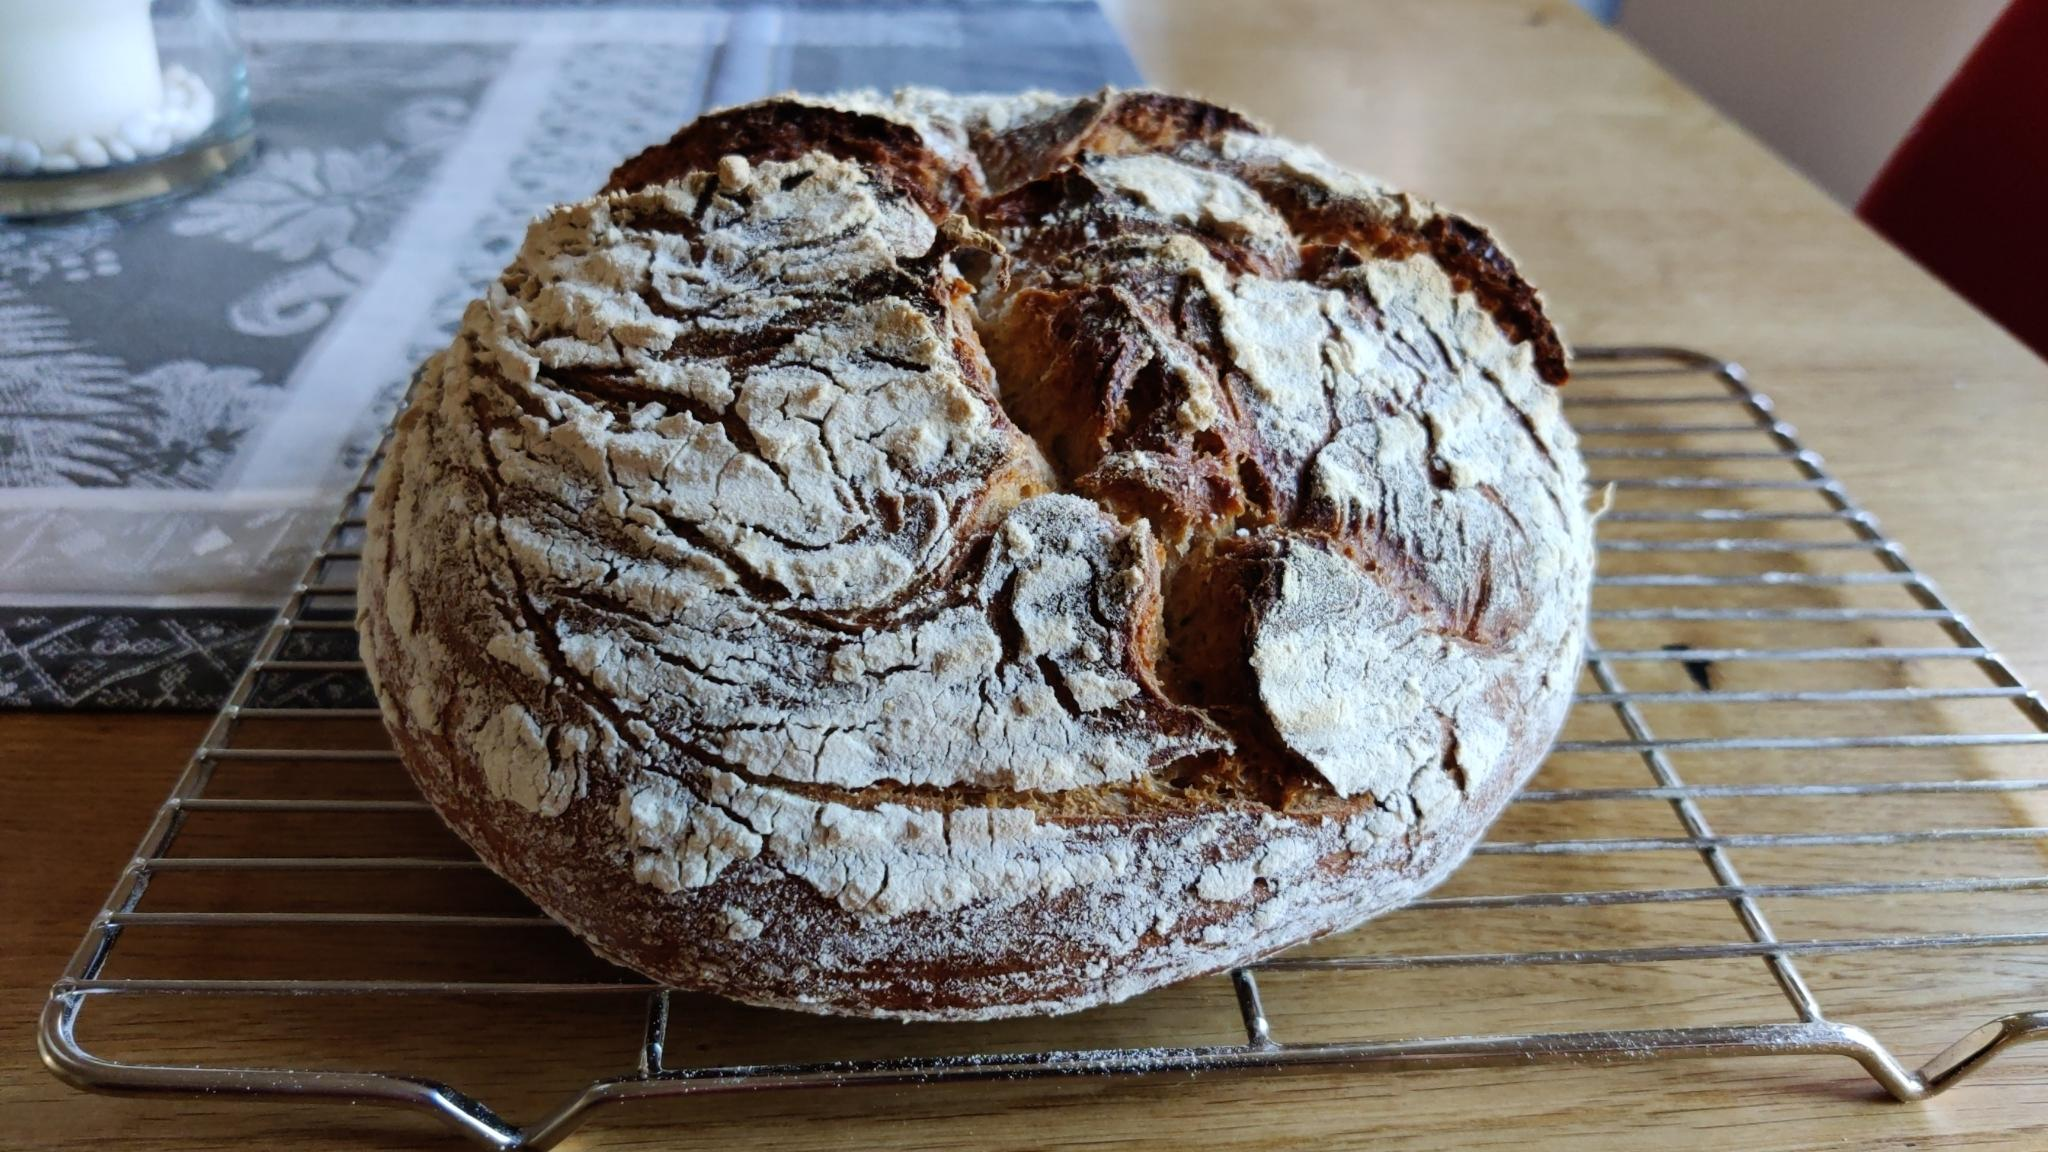
\includegraphics[width=0.7\linewidth]{Bilder/JulesSchwester}
%    \caption{Focaccias aus zwei Rezepten}
%    \label{fig:auffrischbrotJulesSchwester}
%\end{figure}

\subsection*{Zeitplan}
\begin{tabular}{ r @{ Uhr \phantom{bla} } l}
    \toprule
    \multicolumn{1}{c @{\phantom{ bla }}}{Zeit} & \multicolumn{1}{@{}l}{Aktion}   \\ \midrule
    00:00                                       & \Gls{Autolyse}                 \\
    00:30                                       & \Gls{Hauptteig}                 \\
    00:45                                       & \Gls{Stockgare}  Raumtemperatur   \\
    06:45                                       & \Gls{Stockgare}  Kühlschrank mindestens  \\
    12:45                                       & \Gls{Formen} und \Gls{Stueckgare}     \\
    15:45                                       & \Gls{Backen}                          \\
    16:20                                       & fertig                  \\ 
    \bottomrule
\end{tabular}


\subsection*{Zubereitung}

\subsubsection*{\Gls{Autolyse}}
\begin{tabular}{r l}
    350 g & kühles Wasser\\
    500 g & Tipo 00
\end{tabular}\\

Kurz, aber gründlich vermischen.
Für 30 Minuten abgedeckt quellen lassen.

\subsubsection*{\Gls{Hauptteig}}
\begin{tabular}{r l}
           + & Autolyse                               \\
        50 g & Lievito Madre (maximal 12 Stunden alt) \\
         5 g & Honig                                  \\
        15 g & Olivenöl                               \\
        20 g & Salz                                   \\
         2 g & Hefe                                   \\
         2-3 & Knoblauchzehe                          \\
    1 Zweig & Rosmarin gehackt
\end{tabular}\\

Lievito Madre (LM), Hefe und Honig zur Autolyse geben und für 10 Minuten mit geringer Stufe kneten. Salz, Knoblauch, Rosmarin und Olivenöl zugeben, für 3–5 Minuten mit höherer Stufe aus kneten.



\subsubsection*{\Gls{Stockgare}}
Den Teig auf leicht geölter Backfolie in Teigwanne bei Raumtemperatur abgedeckt etwa 10-12 Stunden Gare (erst 6-8 Stunden und dann in den Kühlschrank) stellen. Nach 60 und 120 Minuten dehnen und falten.

\subsubsection*{Formen}
Backpapier/Dauerbackfolie auslegen. Den Teig darauf geben und mit den Händen etwas Olivenöl auf die Teigoberfläche auftragen. 
\subsubsection*{\Gls{Stueckgare}}
Locker abgedeckt für etwa 3 Stunden zur Gare stellen. Mit 40 g Olivenöl 40g Wasser und einem halben Teelöffel Salz mischen und bestreichen . Mulden eindrücken und belegen (Tomaten, Rosmarin und Oliven)

\subsubsection*{Backen}
Bei 230 Grad in den vorgeheizten Ofen. Dampfen. Nach 10 Minuten abdampfen und für weitere 20 Minuten auf 200 Grad reduzieren.


\section{Dinkel Karotten Brot}  \index{Brot!Dinkel}\index{Brot!Möhren}\index{Brot!Lievito Madre}\index{Brot!Kastenbrot}

\todo{Sonja Bauer 176 }
%HAUP T TEIG
%250–280 g Wasser, kühl
%( je nach Saftigkeit der Karotten)
%1 g
%Frischhefe
%0,8 g*
%Acerola-Pulver (optional)
%150 g
%Joghurt, kalt
%150 g
%Möhren, grob geraspelt
%10 g
%inaktives Backmalz/
%Honig
%500
%Dinkelvollkornmehl
%125 g
%gemischte Saaten**,
%geröstet
%12 g
%Salz
%10 g
%Rapsöl
%ZU S ÄT ZL I C H
%gemischte Saaten
%
%Hefe und Acerola-Pulver in dem Wasser auflösen.
%Danach alle Zutaten für den Hauptteig (außer Salz +
%Rapsöl) hinzufügen und für 8–10 Minuten mit geringer
%Stufe kneten. In den letzten 2 Minuten Salz und Rapsöl
%zugeben.
%O D E R : Für 5–6 Minuten bei geringer Stufe in der
%Küchenmaschine mit einem Rührelement mit Gummi-
%lippe mischen. In der letzten Minute Salz und Rapsöl
%zugeben.
%Ohne Hefe:
%Statt 1 g Frischhefe können 30 g vom Weizen-/Rog-
%gen-Anstellgut (ASG) oder Lievito Madre (LM) aus dem
%Kühlschrank ver wendet werden – das ASG/LM sollte
%sehr aktiv sein. Für 10–12 Stunden bei 22–24° C zur
%Stockgare stellen.
%
%IN DIE K A STENFORM GEBEN
%Den Teig in eine gefettete und mit reichlich Saaten ausgestreute/mit Dauerbackfolie ausge-
%legte Kastenform füllen. Teigoberfläche mit einem angefeuchteten Teigschaber glattstrei-
%chen und mit Saaten bestreuen. Die Kastenform ist gut zur Hälfte gefüllt.
%
%9 –1 1 S T D.
%2 0 –2 2° C
%S T Ü C KG A R E
%ZIEL: ca. 1 cm unter dem Rand
%Abgedeckt für 9–11 Stunden bei Raumtemperatur zur Gare stellen.
%Der Teig soll etwa knapp den Rand der Form erreichen.
%6 0 M IN .
%2 3 0° C
%2 0 0° C
%BACKEN
%Backofen rechtzeitig mit einem Backstahl oder Backstein auf 230° C
%Ober-/Unterhitze vorheizen.
%Für insgesamt 60 Minuten ohne Schwaden backen. Nach 10 Minuten die Temperatur auf
%200° C reduzieren. Für die letzten 10 Minuten aus der Form nehmen und zu Ende backen.


\section{Vollkornprotz}  \index{Brot!Dinkel}\index{Brot!Weizen}\index{Brot!Roggen}\index{Brot!Buttermilch}\index{Brot!Lievito Madre}\index{Brot!Roggensauerteig}\index{Brot!Kastenbrot}

\begin{figure}[H]
    \centering
    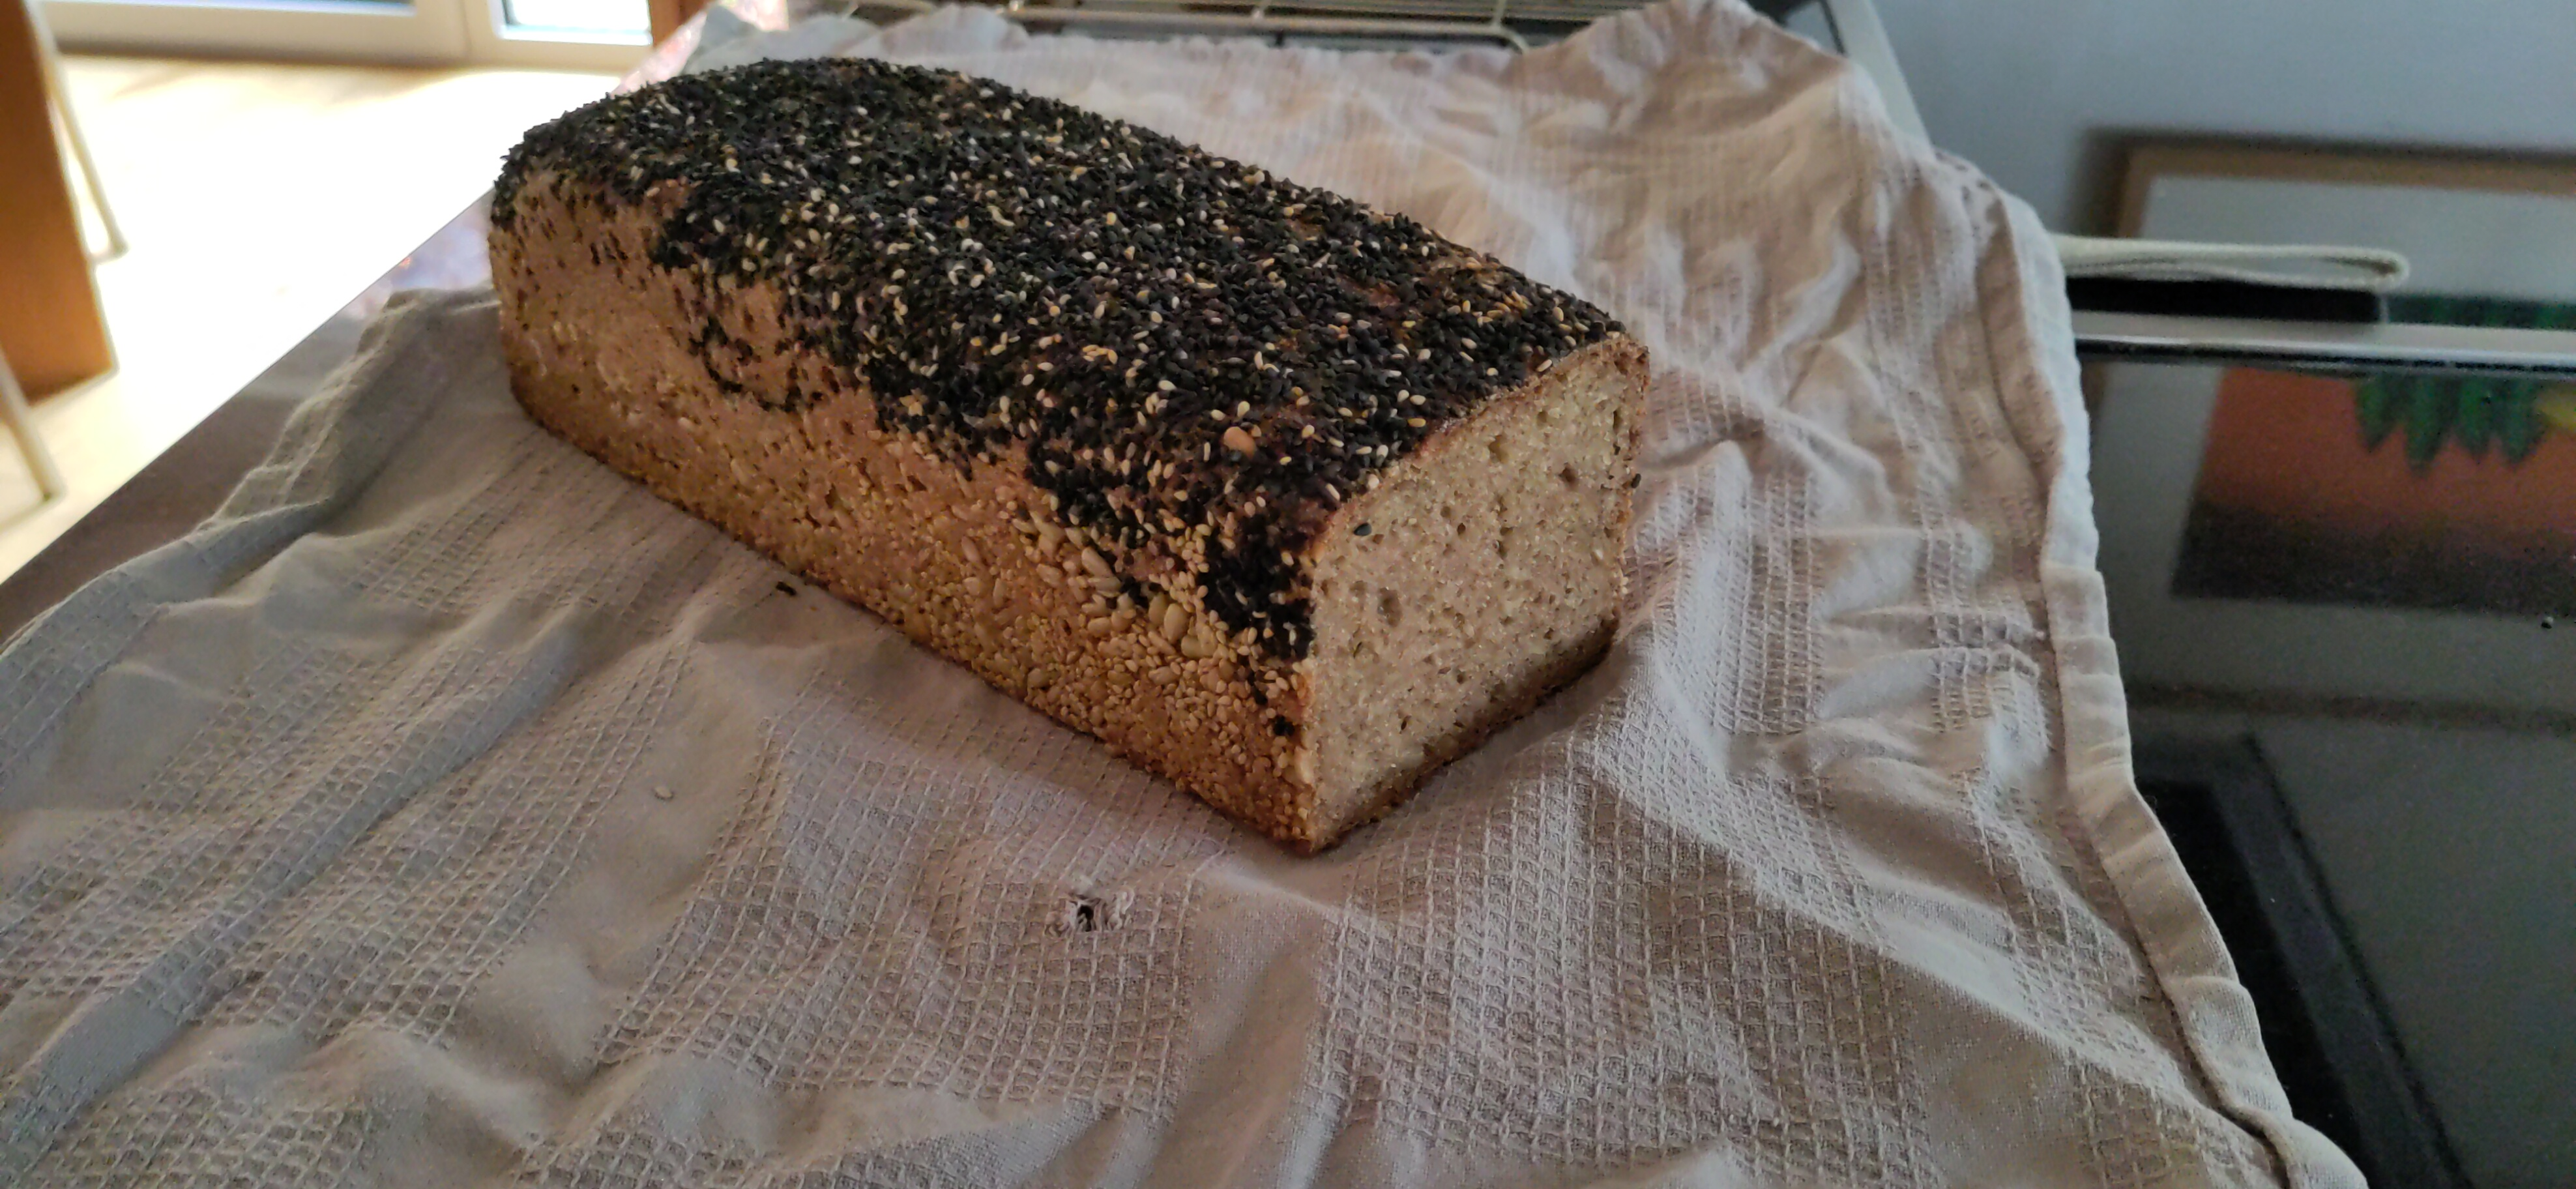
\includegraphics[width=0.7\linewidth]{Bilder/Vollkornprotz}
    \caption{Vollkornprotz mit schwarzem Sesam}
    \label{fig:vollkornprotz}
\end{figure}
 
 
\subsection*{Hauptteig}
\begin{tabular}{r l}
          40 g & Roggensauerteig oder Lievito Madre (+20 g Wasser) \\
         400 g & Buttermilch, kalt                                 \\
         140 g & Wasser, 40° C                                     \\
          10 g & Rübensirup                                        \\
         350 g & Weizenvollkornmehl                                \\
         100 g & Dinkelvollkornmehl                                \\
          50 g & Roggenvollkornmehl                                \\
         0,8 g & Acerola-Pulver                                    \\
          60 g & Sonnenblumenkerne, geröstet                       \\
          20 g & Sesam, geröstet                                   \\
          12 g & Salz                                              \\
          10 g & Olivenöl                                          \\
    zusätzlich & Sonnenblumenkerne und Sesam zum Streuen
\end{tabular}\\

\subsection*{Zubereitung}

\begin{enumerate}
    \item [\Gls{Hauptteig}]  Buttermilch und Wasser mischen. Danach alle Zutaten (das ASG/LM sollte sehr aktiv sein.) für den Hauptteig (außer Salz + Speiseöl) für 8–10 Minuten mit geringer Stufe kneten. Danach 2 Minuten schneller kneten, dabei Salz und Olivenöl zugeben. 
    \item [\Gls{Stueckgare}] 
    Den Teig in eine gefettete und mit reichlich Saaten ausgestreute Kastenform füllen. Teigoberfläche glattstreichen und mit Saaten bestreuen. Die Kastenform ist etwa zur Hälfte gefüllt.\\
    Für 10–12 Stunden bei 22–24° C (13–15 Stunden bei 21° C) zur Stockgare stellen. 
    \item[\GLS{Backen}]
    Backofen rechtzeitig mit einem Backstahl auf 230°C Ober-/Unterhitze vorheizen. Für insgesamt 60 Minuten ohne Schwaden backen. Nach 10 Minuten die Temperatur auf 200° C reduzieren. Für die letzten 10 Minuten aus der Form nehmen und zu Ende backen.
\end{enumerate}

\section[Urkornkasten]{Urkornkasten \textmd{(siehe \cite[188]{SonjaBauer2021})}}  \index{Brot!Urkornkasten} \index{Buttermilch} \index{Brot!Buttermilch}

\subsection*{Zeitplan}
\begin{tabular}{ r @{ Uhr \phantom{bla} } l}
    \toprule
    \multicolumn{1}{c @{\phantom{ bla }}}{Zeit} & \multicolumn{1}{@{}l}{Aktion} \\ \midrule
    00:00                                       & Anstellgut Roggen             \\
    04:00                                       & \Gls{Hauptteig}               \\
    04:15                                       & \Gls{Stueckgare}              \\
    14:45                                       & Vorheizen                     \\
    15:15                                       & \Gls{Backen}                  \\
    16:15                                       & fertig                        \\ \bottomrule
\end{tabular}

\subsection*{Zutaten}
Zweiter Wert für kleinere Backform (ca. 750 g)

\begin{tabular}{r l}
          30 / 22,5 g & aufgefrischt Roggensauerteig oder Lievito Madre (+15 g Wasser) \\
         250 / 187,5  g & Buttermilch                                                    \\
         300 / 225 g & Wasser, 40° C                                                  \\
          10 / 7,5 g & inaktives Backmalz                                             \\
         300 / 225 g & Dinkelvollkornmehl                                             \\
         100 / 75 g & Dinkelmehl  630                                                \\
          50 / 37,5 g & Roggenvollkornmehl                                             \\
          50 / 37,5 g & Waldtaudenroggenmehl                                           \\
          50 / 37,5 g & kernige Haferflocken                                           \\
         0,8 / 0,6 g & Acerola-Pulver                                                 \\
           3 / 2,25 g & Flohsamen                                                      \\
          30 / 22,5 g & Sonnenblumenkerne, geröstet                                    \\
          20 / 15 g & Sesam, geröstet                                                \\
          12 / 9 g & Salz                                                           \\
          10 / 7,5 g & Rapsöl                                                         \\
    zusätzlich & Haferflocken Sonnenblumenkerne und Sesam zum Streuen
\end{tabular}\\

\subsection*{Zubereitung}
\begin{enumerate}
    \item  [\Gls{Hauptteig}]  Wasser und Buttermilch mischen, Roggen-Anstellgut und das Acerola-Pulver darin auflösen. Danach alle Zutaten für den Hauptteig (außer Salz + Öl) hinzufügen und für 8–10 Minuten mit geringer Stufe kneten. In den letzten 2 Minuten Salz und Öl zugeben.
    \item [\GLS{Formen}] Den Teig in eine gefettete und mit Haferflocken, Sonnenblumenkerne und Sesam ausgestreute ausgelegte Kastenform füllen. Teigoberfläche mit einem angefeuchteten Teigschaber glattstreichen und mit Haferflocken, Sonnenblumenkernen und
    Sesam bestreuen. Die Kastenform ist etwa zur Hälfte gefüllt.
    \item [\Gls{Stueckgare}] Abgedeckt für 10–12 Stunden bei warmer Raumtemperatur (22–24° C) zur Gare stellen. Der Teig soll etwa knapp den Rand der Form erreichen.
    \item [\Gls{Backen}] Backofen rechtzeitig mit einem Backstahl oder Backstein auf 230° C Ober-/Unterhitze vorheizen. \\
    Für insgesamt 60 Minuten ohne Schwaden backen. Nach 10 Minuten die Temperatur auf
    200° C reduzieren. Für die letzten 10 Minuten aus der Form nehmen und zu Ende backen. 
\end{enumerate}



\section[Mischbrot 50/50]{Mischbrot 50/50 \textmd{(siehe \cite[130]{SonjaBauer2021})}}  \index{Brot!Mischbrot 50/50} \index{Malzbier} \index{Brot!vegan!Mischbrot}
%\begin{figure}[H]
%%    \centering
%%    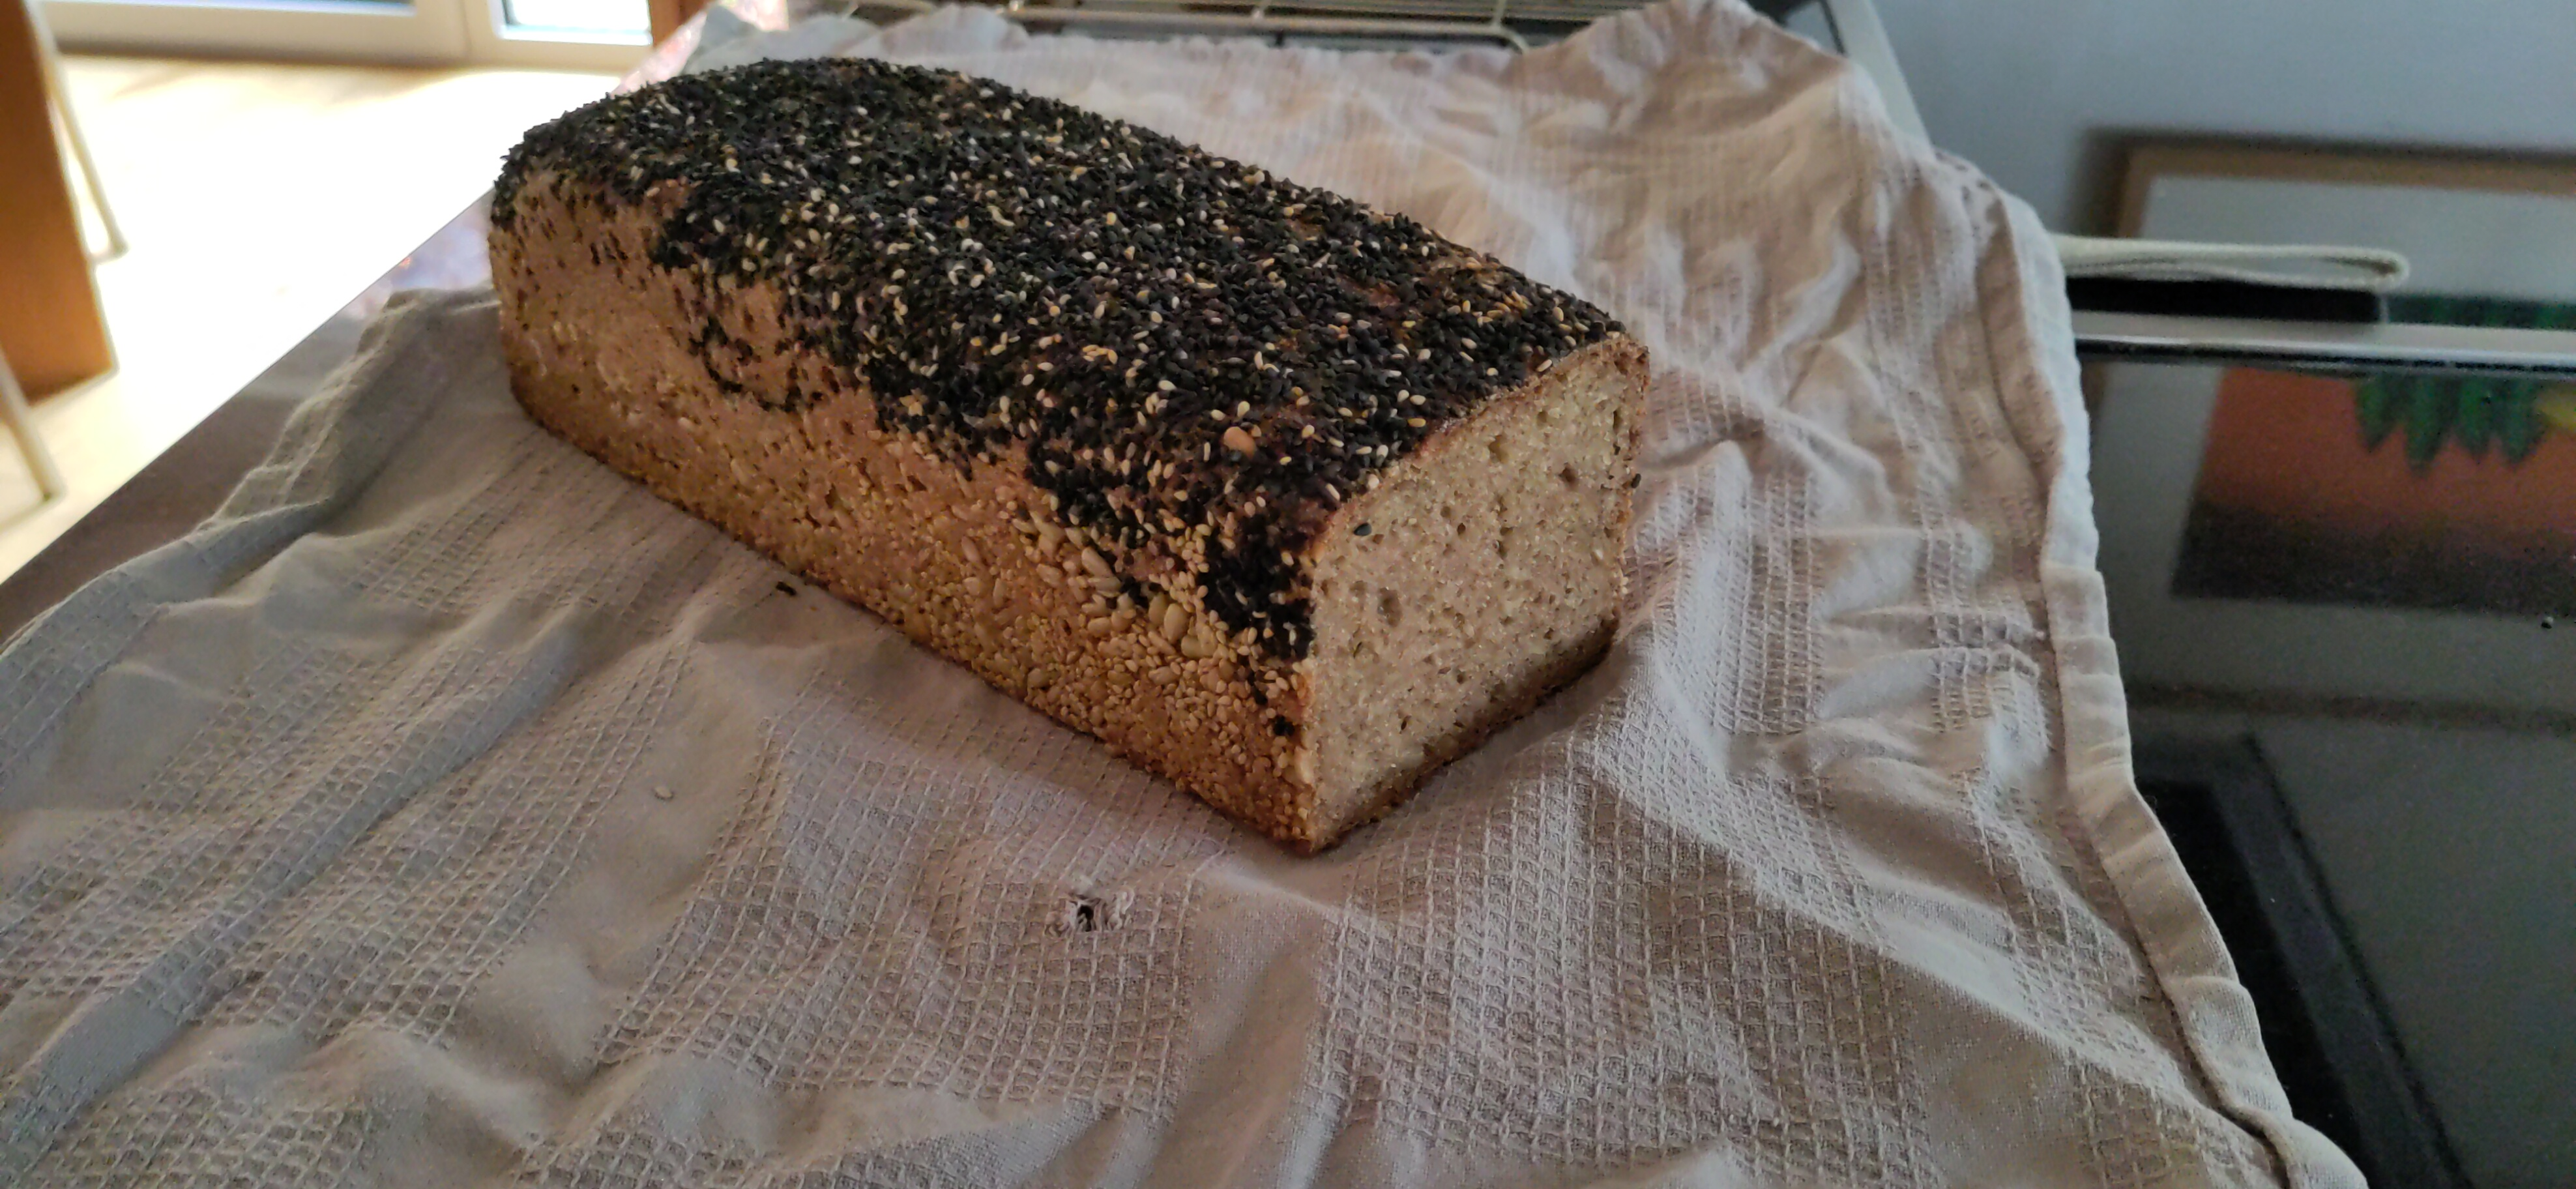
\includegraphics[width=0.7\linewidth]{Bilder/Vollkornprotz}
%%    \caption{Vollkornprotz mit schwarzem Sesam}
%%    \label{fig:vollkornprotz}
%\end{figure}

\subsection*{Zeitplan}
\begin{tabular}{ r @{ Uhr \phantom{bla} } l}
    \toprule
    \multicolumn{1}{c @{\phantom{ bla }}}{Zeit} & \multicolumn{1}{@{}l}{Aktion}      \\ \midrule
    00:00                                       & \Gls{Sauerteig} schnell  / langsam \\
    03:00 / 11:00                               & \Gls{Autolyse}                     \\
    04:00 / 12:00                               & \Gls{Hauptteig}                    \\
    04:20 / 12:20                               & \Gls{Stockgare}                    \\
    06:20 / 14:20                               & Formen + \Gls{Stueckgare}          \\
    07:50 / 15:50                               & Backen                             \\
    08:40 / 16:40                               & fertig                             \\ \bottomrule
\end{tabular}
%
\subsection*{Zutaten}
\begin{tabular}{r l}
    50\;g / 7\;g g & Roggen ASG               \\
             25\;g & Roggen Vollkorn          \\
            200\;g & Roggen 1150              \\
            150\;g & Malzbier                 \\
             60\;g & Weizen Tipo 00           \\
             60\;g & Weizen 550               \\
            130\;g & Weizen 1050              \\
              30 g & Zucker                   \\
             12\;g & Salz                 \\
             2\; g & Frischhefe               \\
\end{tabular}\\

\subsection*{Zubereitung}
\begin{enumerate}
    \item [\Gls{Sauerteig}] Mild im Aroma\\ \textbf{Zutaten:}\\
    \begin{tabular}{r l}
        50\;g & Roggen ASG      \\
        25\;g & Roggen Vollkorn \\
        25\;g & Roggen 1150     \\
        40\;g & Wasser
    \end{tabular}

    Alle Zutaten gründlich mischen. Für 2–4 Stunden bei 26--28°\;C reifen lassen.
    
    \item [\Gls{Sauerteig}] Kräftig im Aroma\\ \textbf{Zutaten:}\\
    \begin{tabular}{r l}
        6\;g & Roggen ASG      \\
        35\;g & Roggen Vollkorn \\
        40\;g & Roggen 1150     \\
        75\;g & Wasser
    \end{tabular}

    Alle Zutaten gründlich mischen. Für 10--12 Stunden bei 22°\;C reifen lassen.

    \item [\Gls{Autolyse}]  \textbf{Zutaten:}\\
    \begin{tabular}{r l}
        160\;g & Wasser 30°\;C  \\
        150\;g & Malzbier       \\
         60\;g & Weizen Tipo 00 \\
         60\;g & Weizen 550     \\
        130\;g & Weizen 1050
    \end{tabular}

    Alles kurz, aber gründlich mischen. Für 60 Minuten abgedeckt quellen lassen.

    \item [\Gls{Hauptteig}]  \textbf{Zutaten:}\\
    \begin{tabular}{r l}
        + & Autolyse  \\
        + & Sauerteig       \\
        2\;g & Hefe \\
        13\;g & Roggen 1150     \\
        12\;g & Salz
    \end{tabular}

    Alle Zutaten des Hauptteigs für 5--8 Minuten bei langsamer Geschwindigkeit mischen. 

    \item [\Gls{Stockgare}] Abgedeckt 90–120 Minuten bei 25–27° C zur Gare stellen.

    \item [\Gls{Formen}] Auf der bemehlten Arbeitsfläche rund wirken. Mit dem Schluss nach unten in ein bemehltes Gärkörbchen geben.
    \item[\Gls{Stueckgare}] Abgedeckt für 90 Minuten bei Raumtemperatur zur Gare stellen.
    \item[\Gls{Backen}] 250° C Ober–/Unterhitze vorheizen.\\
    Teigling aus dem Gärkörbchen stürzen und einschießen. Sofort schwaden und für insgesamt 50 Minuten backen. Nach 10 Minuten den Dampf ablassen und die Temperatur auf 210° C reduzieren.
\end{enumerate}

\section[Rosinenbrot]{Rosinenbrot \textmd{(siehe \cite{sonjarosinenbrot2023})} }  \index{Brot!Rosinen}\index{Brot!Weizen 550}\index{Brot!Lievito Madre}
\subsection*{Zeitplan}
\begin{tabular}{ r @{ Uhr \phantom{bla} } l}
    \toprule
    \multicolumn{1}{c @{\phantom{ bla }}}{Zeit} & \multicolumn{1}{@{}l}{Aktion}         \\ \midrule
    00:00                                       & \Gls{Quellstueck} \Gls{Auffrischen}  \\
    04:00                                       & \Gls{Hauptteig}                       \\
    04:20                                       & \Gls{Stockgare}                       \\
    08:20                                       & Formen und \Gls{Zwischengare}         \\
    09:00                                       & \Gls{Stueckgare} Kühlschrank          \\
    20:00                                       & Akklimatisieren                       \\
    20:10                                       & Backen                                \\
    20:50                                       & fertig                                \\ \bottomrule
\end{tabular}


%\begin{figure}[H]
%%    \centering
%%    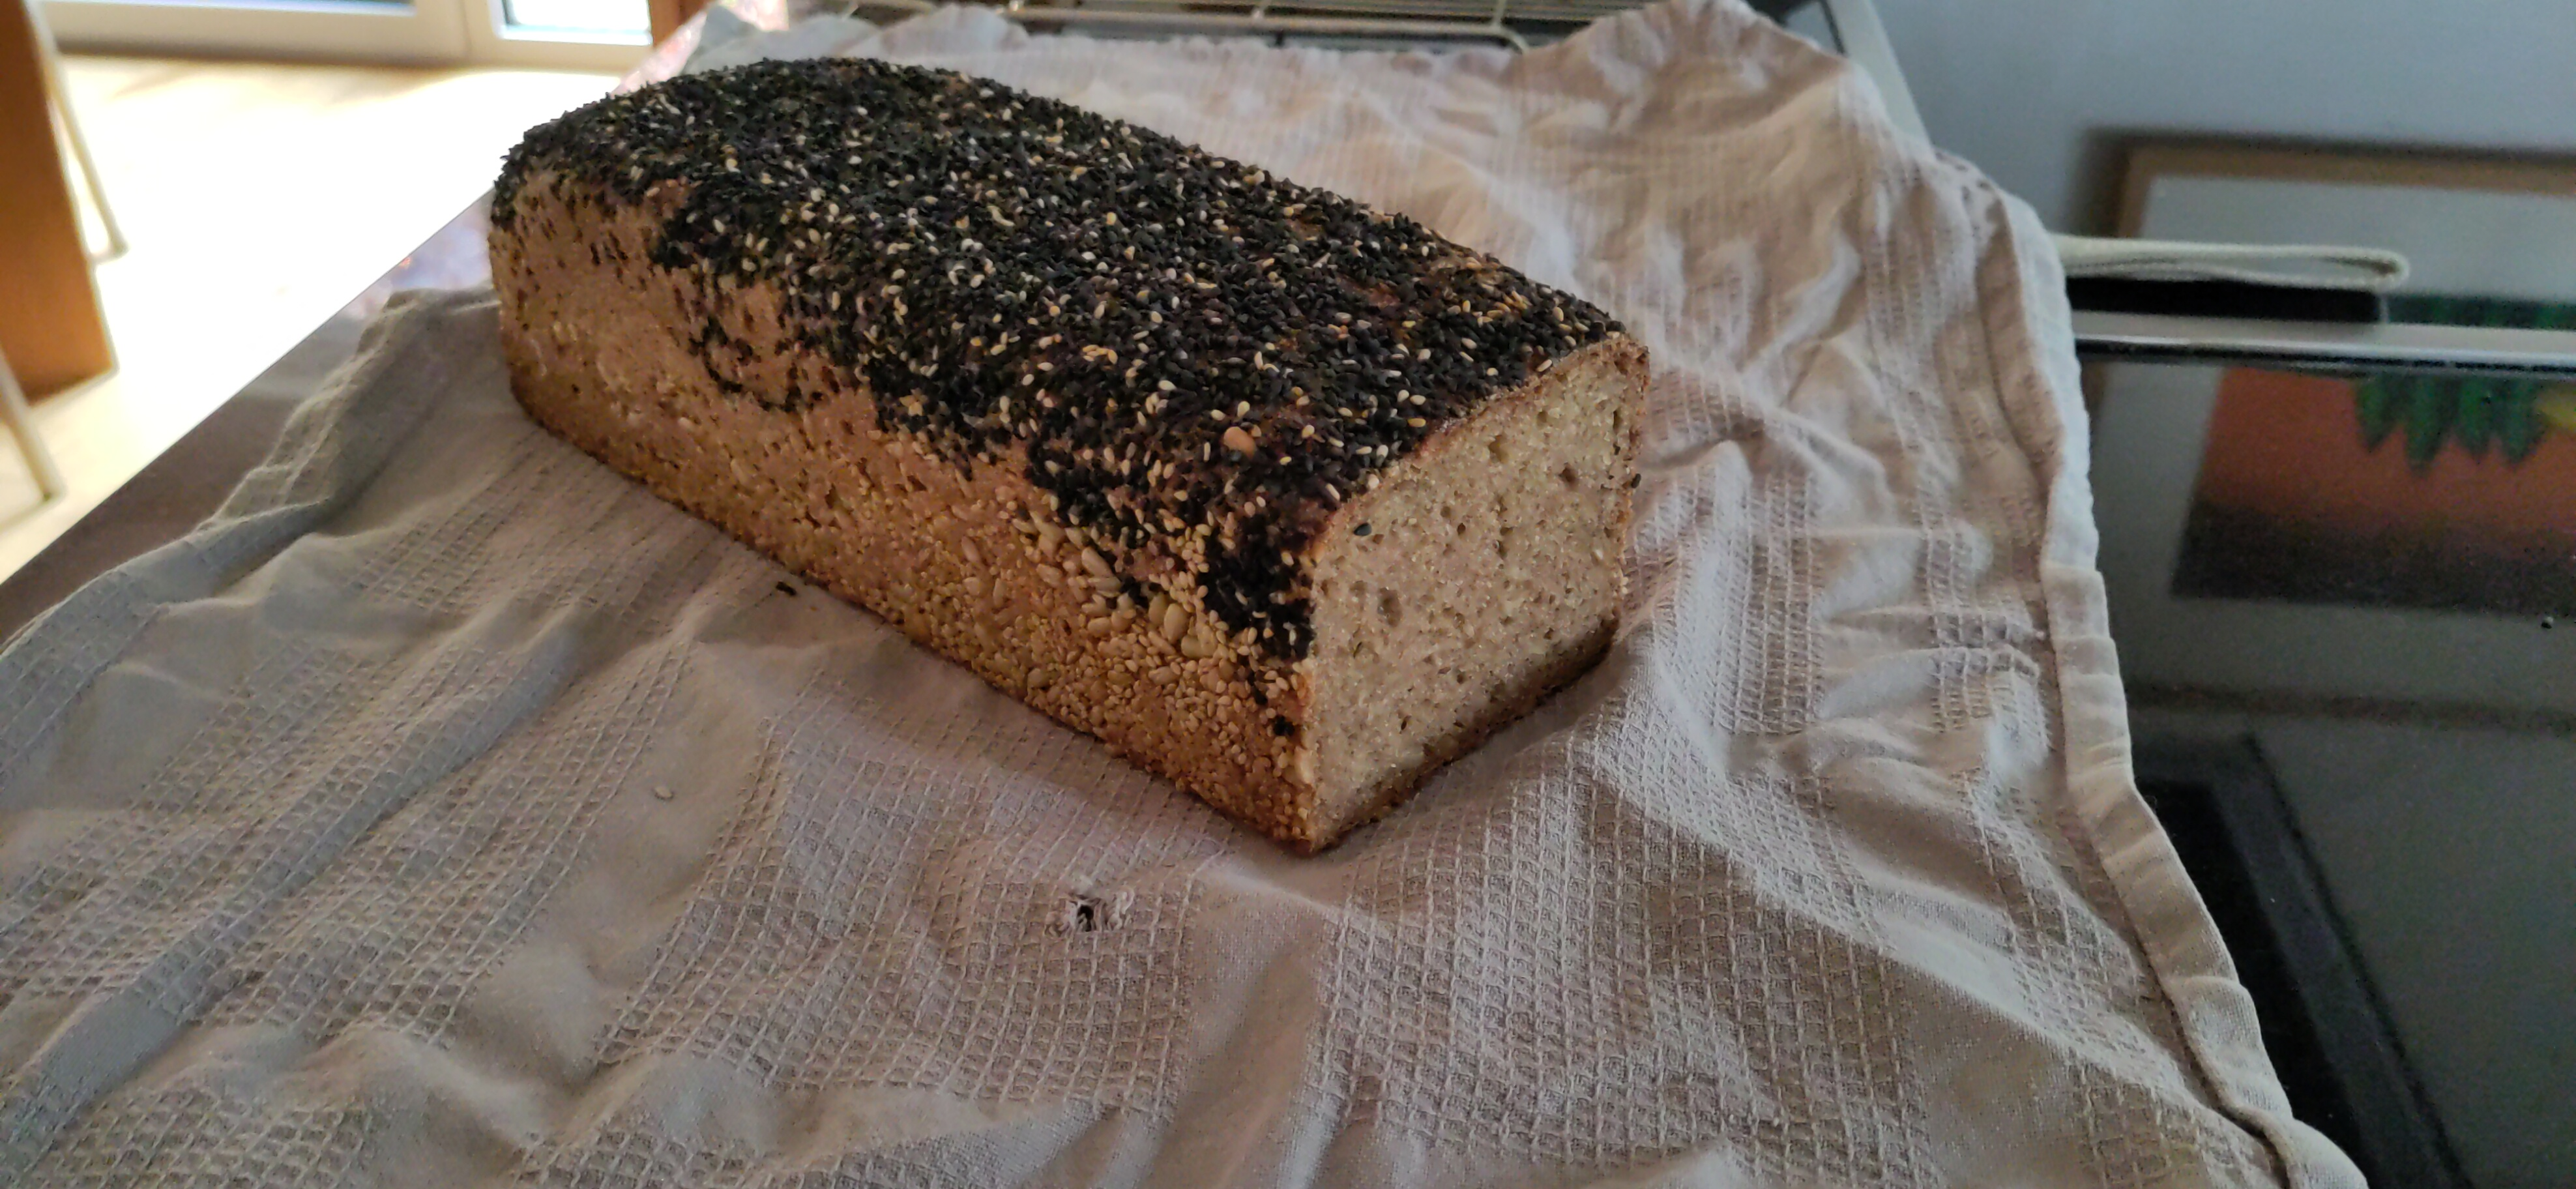
\includegraphics[width=0.7\linewidth]{Bilder/Vollkornprotz}
%%    \caption{Vollkornprotz mit schwarzem Sesam}
%%    \label{fig:vollkornprotz}
%\end{figure}
%
%
\subsection*{Zutaten}
\begin{tabular}{r l}
          475 g & Weizenmehl Type 550          \\
          320 g & Milch (ca. 3,5\% Fett)       \\
          120 g & Rosinen                      \\
           75 g & aufgefrischter \Gls{LievitoMadre} \\
           60 g & Butter                       \\
           60 g & Milch                        \\
           30 g & Zucker Vanillezucker         \\
           30 g & Zucker                       \\
            8 g & Salz                         \\
            5 g & Frischhefe                   \\
              2 & Ei(er), Gr. M                \\
    0.5 Zitrone & Abrieb Versuch weglassen
\end{tabular}\\



\subsection*{Zubereitung}
\begin{enumerate}
    \item [\Gls{Auffrischen}] \textbf{Zutaten:}\\
         Für aufgefrischten Lievito Madre siehe \vref{sec:Lievito Madre},
    
    \item [\Gls{Quellstueck}] \textbf{Zutaten:}\\
        \begin{tabular}{r l}
            120 g  & Rosinen  \\
            60 g &  Milch  
        \end{tabular}
        
        Die Rosinen mit der Milch (ggf, 20 g durch Rum ersetzen) mischen und abgedeckt mindestens 4 Stunden oder über Nacht (im Kühlschrank) einweichen.
    \item  [\Gls{Hauptteig}] \textbf{Zutaten:}\\
        \begin{tabular}{r l}
            475 g & Weizenmehl Type 550                   \\
            260 g & Milch (ca. 3,5\% Fett)                \\
            75 g & aufgefrischter Lievito Madre          \\
            60 g & Butter                                \\
            30 g & Zucker Vanillezucker                  \\
            30 g & Zucker                                \\
            8 g & Salz                                  \\
            5 g & Frischhefe                            \\
            1 & Ei(er), Gr. M                         \\
            0.5 Zitrone & Abrieb Versuch weglassen              \\
            & Quellstück (abgetropft)               \\
            & abgetropfte Flüssigkeit als Bassinage
        \end{tabular}
        
        Alle Zutaten für den Teig (außer Butter und Salz) etwa 10 Minuten bei langsamer Geschwindigkeit in der Küchenmaschine kneten.\\
        Anschließend etwa 5–8 Minuten bei höherer Geschwindigkeit weiter kneten, dabei portionsweise die Butter und das Salz hinzufügen. Dabei nach Bedarf noch bis zu 20 g der Flüssigkeit des Quellstücks mit einkneten.\\
        Zum Schluss das abgetropfte Quellstück kurz mit der Hand oder bei langsamer Geschwindigkeit mit der Küchenmaschine unter den Teig kneten.
    \item  [\Gls{Stockgare}] Den Teig in einer leicht geölten Schüssel oder Teigwanne abgedeckt bei
    Raumtemperatur etwa 3 bis 4 Stunden bis zur guten Verdopplung reifen lassen.\\
    Dabei nach 1 Stunde dehnen und falten.
    \item [\GLS{Formen}] Eine 1-kg-Brotbackform (23 × 11 × 9,5 cm) einfetten und leicht bemehlen.\\
     Den Teig auf der leicht bemehlten Arbeitsfläche (z. B. mit Weizendunst) länglich formen und in die vorbereitete Kastenform geben.
    \item [\Gls{Stueckgare}] Abgedeckt 30–40 Minuten bei Raumtemperatur anspringen lassen, danach für etwa 10–12 Stunden im Kühlschrank bei 5 °C weiter reifen lassen.
    \item [Backen] \textbf{Zutaten:}\\
    \begin{tabular}{r l}
        1 & Ei     \\
        10g & Milch  \\
        1 Prise & Zucker \\
        1 Prise & Salz
    \end{tabular}
    
    Den Backofen rechtzeitig auf 210 °C Ober-/Unterhitze vorheizen.\\
    Für die Eistreiche alle Zutaten gründlich miteinander verquirlen und danach gerne durch ein Sieb streichen. \\
    Die Kastenform aus dem Kühlschrank nehmen und den Teig mit der Eistreiche bestreichen. \\
    Danach einmal längs einschneiden und in den vorgeheizten Backofen einschießen und insgesamt etwa 40–45 Minuten backen. Je nach Backform und
    Backofen kann die sich die Backzeit etwas verlängern, auf 50 bis max. 60 Minuten; Die Kerntemperatur sollte 90–93 °C erreichen.\\
    Dabei nach 1–2 Minuten Backzeit verzögert schwaden und die Temperatur auf 180 °C Ober-/Unterhitze  reduzieren.\\
    Den Schwaden während der gesamten Backzeit nicht ablassen. \\
    Nach dem Backen aus der Kastenform nehmen, mit einem leicht feuchtem Geschirrtuch bedeckt auf einem Rost auskühlen lassen. 
\end{enumerate}



\section{Mohnkruste}  \index{Brot!Mohn}\index{Brot!Weizen}\index{Brot!Lievito Madre}

%%\begin{figure}[H]
%%%    \centering
%%%    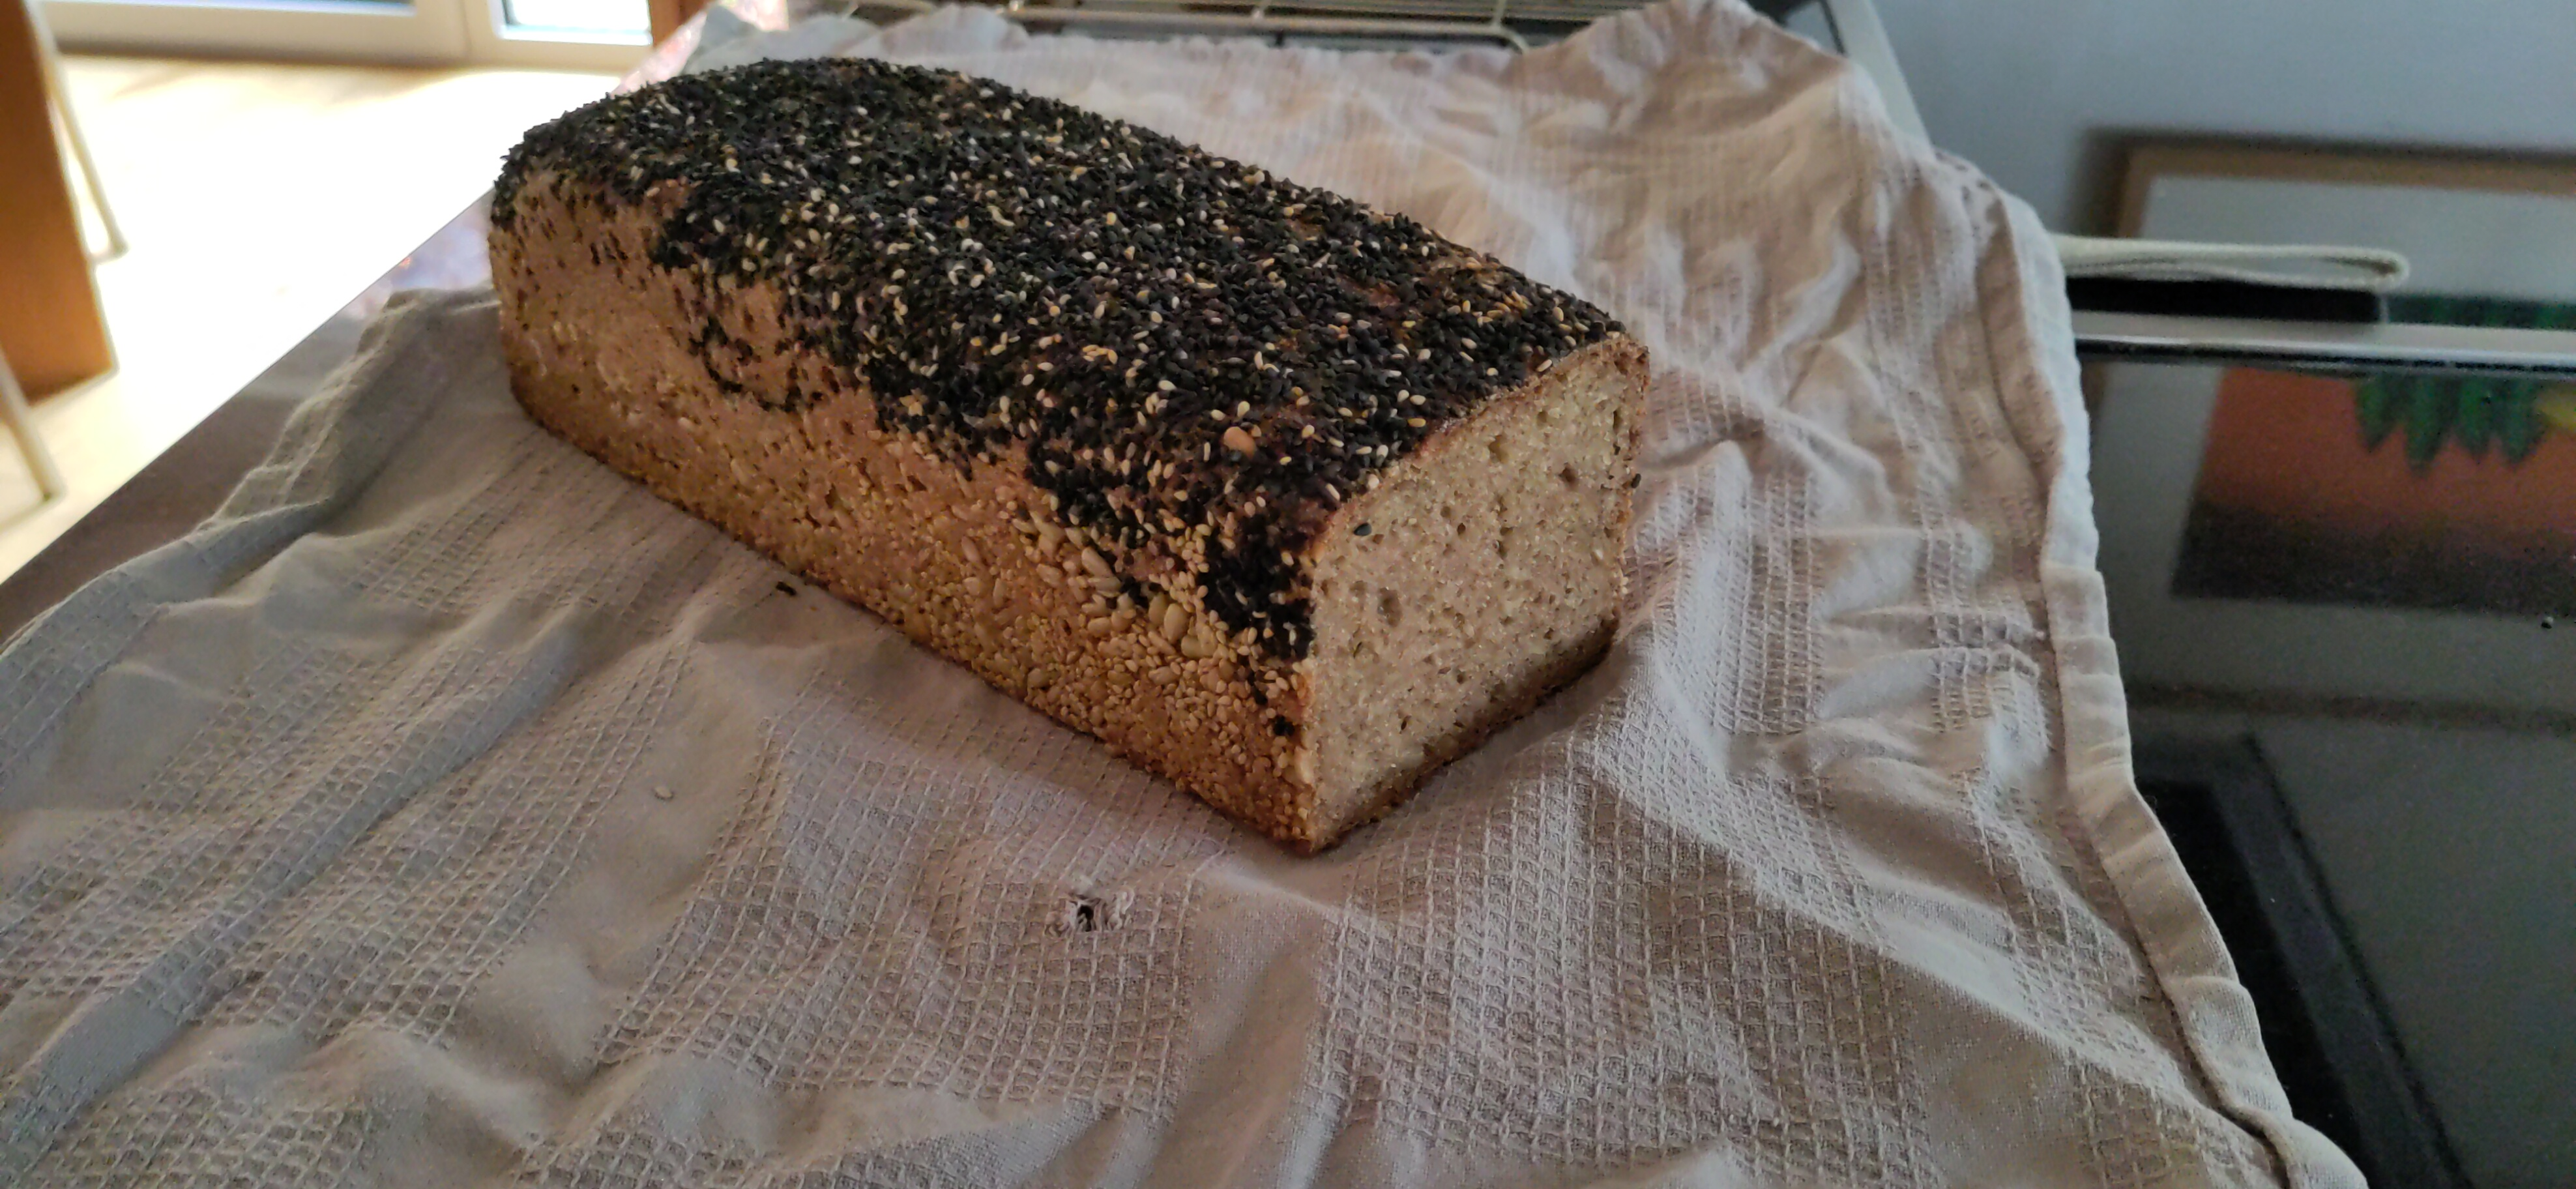
\includegraphics[width=0.7\linewidth]{Bilder/Vollkornprotz}
%%%    \caption{Vollkornprotz mit schwarzem Sesam}
%%%    \label{fig:vollkornprotz}
%%\end{figure}
%%
%%
%%\subsection*{Hauptteig}
%A U T O LY S E
%350 g
%350 g
%100 g
%50 g
%Wasser, kühl
%Weizenmehl T 550
%Weizenmehl T 1050
%Weizenvollkornmehl
%HAUP T TEIG
%+
%1 g
%10 g
%12 g
%30 g
%± 30 g
%Autolyse
%Frischhefe
%Honig
%Salz
%Mohn
%Wasser bei Bedarf
%(Bassinage)
%ZU S ÄT ZL I C H
%Mohn
%
%%
%%\subsection*{Zubereitung}
%Kurz, aber gründlich vermischen.
%Für 30 Minuten abgedeckt quellen lassen.
%M E N G E : ca . 9 2 0 g •
%TE I GTE M P E R A TU R : 24–26° C
%Alle Zutaten (außer Salz + Bassinage) für 8–10 Minuten mit
%geringer Stufe kneten. Salz zugeben, für 3–5 Minuten
%mit höherer Stufe auskneten und bei Bedarf portions-
%weise bis zu 30 g Wasser (Bassinage) mit einkneten.
%Ohne Hefe:
%Statt 1 g Hefe können auch 40 g Lievito Madre
%(LM, aufgefrischt) ver wendet werden.
%Für 10–12 Stunden bei 22–24° C zur Stockgare stellen.
%
%M O HNK RUS T E
%Einfaches Weizenbrot mit Mohn
%1 0 –1 2 S T D.
%2 0 –2 2° C
%D + F:
%4 5 | 90 MIN.
%S T O C KG A R E
%Z I E L : etwa Verdopplung
%Abgedeckt für 10–12 Stunden bei Raumtemperatur zur Gare stellen.
%Nach 45 und 90 Minuten dehnen und falten (D + F) .
%FORMEN
%Auf der bemehlten Arbeitsfläche schonend rund wirken und mit
%dem Schluss nach oben in ein bemehltes Gärkörbchen geben.
%6 0 –9 0 M IN .
%2 0 –2 2° C
%ODER
%1 2–1 4 S T D.
%5 – 6° C
%S T Ü C KG A R E
%Z I E L : k n a p p e G a r e (siehe S. 69)
%Abgedeckt für 60–90 Minuten bei Raumtemperatur zur Gare stellen.
%O D E R : Ohne Anspringen für 12–14 Stunden bei 5–6° C im Kühlschrank zur
%Gare stellen. Anschließend ohne Akklimatisieren backen.
%5 0 M IN .
%2 5 0° C
%2 1 0° C
%BACKEN
%Backofen rechtzeitig mit einem Backstahl, Backstein oder Gusstopf auf
%250° C Ober–/Unterhitze vorheizen.



\section[Quarkstuten]{Quarkstuten \textmd{(siehe \cite[296]{SonjaBauer2021})} }  \index{Brot!Quark}\index{Brot!Weizen}\index{Brot!Lievito Madre}
\subsection*{Zeitplan}
\begin{tabular}{ r @{ Uhr \phantom{bla} } l}
    \toprule
    \multicolumn{1}{c @{\phantom{ bla }}}{Zeit} & \multicolumn{1}{@{}l}{Aktion}   \\ \midrule
    -03:30                                      & \Gls{LievitoMadre}              \\
    00:00                                       & \Gls{Hauptteig}                 \\
    00:20                                       & \Gls{Stockgare}                 \\ \midrule
    03:50                                       & Formen und \Gls{Zwischengare}   \\
    04:05                                       & \Gls{Stueckgare} Raumtemperatur \\
    05:50                                       & Backen                          \\
    06:30                                       & fertig                          \\ \midrule
    04:05                                       & \Gls{Stueckgare} Kühlschrank    \\
    15:05                                       & Akklimatisieren                 \\
    15:35                                       & Backen                          \\
    16:15                                       & fertig                          \\ \bottomrule
\end{tabular}

%L I E V I T O M A D R E (LM)
%15 g
%30 g
%30 g
%Wasser, 40° C
%LM
%Weizenmehl T 550
%Z I E L : mindestens Verdopplung
%Lievito Madre mit dem Wasser schaumig aufschlagen.
%Danach mit dem Mehl verkneten. Für 2–4 Stunden bei
%26–30° C reifen lassen.
%HAUP T TEIG
%150 g
%100 g
%+
%5 g
%1
%1
%60 g
%1
%10 g
%500 g
%60 g
%5 g
%± 30 g
%Quark/Topfen, kalt
%Milch, kalt
%LM
%Frischhefe
%Ei (Gr. M) , kalt
%Eiklar, kalt
%Zucker
%unbehandelte Zitrone,
%davon den Schalenabrieb
%Bourbon-Vanillezucker
%Weizenmehl T 550
%Butter, kühl
%Salz
%Milch bei Bedarf
%( Bassinage)
%M E N G E : ca. 1 .0 8 0 g • TE I GTE M P E R A TU R : 2 4 –2 6° C
%Alle Zutaten (außer Butter + Salz + Bassinage) für 10 Mi-
%nuten bei geringer Stufe kneten. Für 5–8 Minuten bei
%höherer Stufe auskneten. Dabei Salz, portionsweise
%die Butter und bei Bedarf noch bis zu 30 g Milch
%(Bassinage) mit einkneten.
%Hinweis:
%Statt Lievito Madre können insgesamt 10 g
%Frischhefe + 50 g Mehl + 25 g Wasser an den
%Hauptteig gegeben werden.
%EISTREICHE
%1
%10 g
%1 Prise
%Eigelb (das übrig gebliebene)
%Milch/Sahne
%Salz + Zucker
%Alle Zutaten kurz verquirlen und bereitstellen.
%ZU S ÄT ZL I C H : Hagelzucker und gehobelte Mandeln

%S T O C KG A R E
%Z I E L : et wa Verdopplung
%Abgedeckt für etwa 3–4 Stunden bei Raumtemperatur zur Gare stellen.
%Nach 60 Minuten dehnen und falten (D + F).
%FORMEN + ZWISCHENGARE
%Kastenform einfetten und leicht bemehlen oder mit Backpapier/Dauerbackfolie auslegen.
%Anschließend den Teig in 2 Teile à ca. 540 g teilen.
%Diese jeweils locker rund wirken und abgedeckt für 10 Minuten ruhen lassen (Zwischengare).
%Danach zu 2 Strängen von etwa 40 cm formen, diese kordelartig ineinander verschlingen
%und in die vorbereitete Backform legen.
%Mit der Eistreiche bestreichen, die restliche Eistreiche kaltstellen.
%S T Ü C KG A R E
%Z I E L : 2– 3 c m ü b e r d e n R a n d d e r F o r m
%Abgedeckt für etwa 90–120 Minuten bei Raumtemperatur zur Gare stellen. Der Teig
%sollte deutlich aufgegangen sein, beziehungsweise im Idealfall 2–3 cm über den Rand
%der Kastenform reichen.
%O D E R : Abgedeckt für 30 Minuten anspringen lassen, danach für etwa 10–12 Stunden
%im Kühlschrank bei 5° C zur Gare stellen. Anschließend für 30–60 Minuten bei Raum-
%temperatur akklimatisieren lassen.
%BACKEN
%Backofen rechtzeitig auf 210° C Ober-/Unterhitze vorheizen.
%Den Teigling erneut mit der Eistreiche einstreichen und mit Hagelzucker und gehobelten
%Mandeln bestreuen. Einschießen und die Temperatur auf 180° C reduzieren.
%Für insgesamt etwa 40 Minuten backen. Bei zu starker Bräunung rechtzeitig abdecken.

\chapter{Auffrischbrote}

\section[Frühstücksbrot]{Frühstücksbrot \textmd{(siehe \cite[227]{SonjaBauer2021})} }  \index{Auffrischbrot!Frühstücksbrot}\index{Brot!Auffrischbrot}\index{Brot!Weizen}\index{Brot!Lievito Madre}

\subsection*{Zeitplan}
\begin{tabular}{ r @{ Uhr \phantom{bla} } l}
    \toprule
    \multicolumn{1}{c @{\phantom{ bla }}}{Zeit} & \multicolumn{1}{@{}l}{Aktion} \\ \midrule
    00:00                                       & \Gls{Hauptteig}               \\
    00:20                                       & \Gls{Stockgare}               \\
    03:50                                       & Formen und \Gls{Zwischengare} \\
    04:35                                       & \Gls{Stueckgare} Kühlschrank  \\
    15:35                                       & Akklimatisieren               \\
    15:50                                       & Backen                        \\
    16:30                                       & fertig                        \\ \bottomrule
\end{tabular}
%
\subsection*{Zutaten}
%\subsubsection*{Alle Zutaten}
\begin{tabular}{r l}
    150 g & Wasser, kühl         \\
    150 g & Milch, kalt     \\
    75g & Lievito Madre \\
    2 g & Frischhefe            \\
    450 g & Weizenmehl T 550     \\
    10 g & Honig            \\
    20 g & Butter kühl \\
    11 g & Salz                  \\
    Zusätzlich & Mohn oder Sesam
\end{tabular}\\

\subsection*{Zubereitung}
\begin{enumerate}
    \item  [\Gls{Hauptteig}]  Alle Zutaten (außer Butter + Salz + Bassinage) für 10 Minuten bei geringer Stufe kneten. Salz und Butter hinzufügen, für 5–8 Minuten bei höherer Stufe auskneten und bei Bedarf portionsweise bis zu 25 g     Wasser (Bassinage) mit einkneten.
    \item [\Gls{Stockgare}] Abgedeckt für 3–4 Stunden bei Raumtemperatur zur Gare stellen. Nach 60 und 120 Minuten dehnen und falten (D + F) . 
    \item [\Gls{Formen}] Den Teig auf der leicht bemehlten Arbeitsfläche zu zwei runden Teiglingen je ca. 450 g formen. Mit dem Schluss nach unten in eine gefettete Kastenform geben. Teiglinge anfeuchten und mit Mohn oder Sesam bestreuen.
    \item [\Gls{Stueckgare}] Abgedeckt 30–40 Minuten bei Raumtemperatur anspringen lassen, danach für etwa 10–12 Stunden im Kühlschrank bei 5 °C weiter reifen lassen.
    \item [\Gls{Backen}] Kastenform aus dem Kühlschrank nehmen. Backofen rechtzeitig mit einem Backstahl 230° C Ober-/Unterhitze vorheizen.Teigling längs einschneiden und einschießen. Sofort schwaden und die Temperatur auf 200° C reduzieren.\\ 
    Für insgesamt 40 Minuten backen. Nach 10 Minuten den Dampf ablassen. Nach dem Backen sofort mit etwas Wasser einsprühen.   
\end{enumerate}



\section{Auffrischbrötchen Julchen}  \index{Brot!Weizen}\index{Brot!Lievito Madre}\index{Auffrischbrot! Brötchen Julchen}
\cite{sonjajulchen2022}
\subsection*{Zeitplan}
\begin{tabular}{ r @{ Uhr \phantom{bla} } l}
    \toprule
    \multicolumn{1}{c @{\phantom{ bla }}}{Zeit} & \multicolumn{1}{@{}l}{Aktion} \\ \midrule
    00:00                                       & \Gls{Fermentolyse}            \\
    00:30                                       & \Gls{Hauptteig}               \\
    00:50                                       & \Gls{Stockgare}               \\
    01:50                                       & \Gls{DehnenUndFalten}         \\
    02:50                                       & \Gls{DehnenUndFalten}         \\
    03:50                                       & \Gls{Formen}                  \\
    04:00                                       & \Gls{Stueckgare}              \\
    04:30                                       & \GLS{Vorheizen}               \\
    05:00                                       & \GLS{Backen}                  \\
    05:20                                       & fertig                        \\ \bottomrule
\end{tabular}


\subsection*{Zutaten}
\subsubsection*{Fermentolyseteig}
\begin{tabular}{r l}
    75 g & Lievito-Madre-Anstellgut\\
    180 g & kalte Vollmilch (oder pflanzliche Alternative)\\
    145 g & kühles Wasser\\
    400 g & Weizenmehl Type 550\\
    50 g & Vollkornmehl nach Wahl\\
\end{tabular}\\
Alles kurz, aber gründlich mischen und für 20−30 Minuten abgedeckt quellen lassen.


\subsubsection*{Hauptteig}
\begin{tabular}{r l}
    & Fermentolyseteig                                      \\
    5 g & Frischhefe (oder 3 g bei kalter Übernachtgare         \\
    10 g & Honig  \\
    11 g & Salz                                                  \\
    10 g & Butter (oder Olivenöl)                                \\
    20 g & Wasser nach Bedarf (Bassinage)                        \\
    & Roggenmehl zum Aufarbeiten (z. B. Type 610 oder 1150)
\end{tabular}\\


\subsection*{Zubereitung}
\begin{enumerate}
    \item [Teig] 
    \begin{itemize}
        \item Die Frischhefe und den Blütenhonig zum Fermentolyseteig geben und für 10 Minuten mit geringer Stufe kneten.
        \item Danach das Salz und die Butter zugeben und für 3–5 Minuten mit höherer Stufe auskneten, dabei bei Bedarf noch bis zu 20 g Wasser mit einkneten. )]
    \end{itemize}
    \item [Stockgare]
    \begin{itemize}
        \item Den Teig in einer leicht geölten Schüssel oder Teigwanne bei Raumtemperatur abgedeckt etwa 3 Stunden bis zur guten Verdopplung reifen lassen, dabei nach 1 und 2 Stunden schonend dehnen und falten (Coil fold).
        \item Variation kalte Stockgare: Für 90 Minuten bei Raumtemperatur (20−22 °C) anspringen lassen. Dabei nach jeweils 45 und 90 Minuten dehnen und falten. Danach für 12−14 Stunden bei 5 °C in den Kühlschrank geben. Anschließend für mindestens 1 Stunde akklimatisieren lassen.
    \end{itemize}
    \item [Formen]
    \begin{itemize}
        \item Den Teig auf der bemehlten Arbeitsfläche in neun Teile mit je etwa 95 g teilen.
        \item Die Teiglinge schonend rund wirken und dabei Roggenmehl in den Teigschluss einarbeiten, damit dieser während der Stückgare nicht verklebt.
        \item Danach mit dem Teigschluss nach unten in ein leicht bemehltes Bäckerleinen oder Geschirrtuch legen und den Stoff zwischen den Teiglingen etwas hochziehen, damit diese gestützt werden.
    \end{itemize}
    \item [\Gls{Stueckgare}]
    \begin{itemize}
        \item Die Teiglinge abgedeckt bei Raumtemperatur (20−22 °C) etwa 60–80 Minuten bis zur knappen Gare reifen lassen.
        \item Variation kalte Stückgare:  Die Teiglinge ohne Anspringen (gut eingepackt, z. B. mit XXL Gefrierbeuteln*) über Nacht 10–12 Stunden in den Kühlschrank bei 4–5 °C reifen lassen. (Die Kühlschranktemperatur bitte unbedingt nachmessen!) Danach ohne Akklimatisieren backen.
    \end{itemize}
    \item [Backen]
    \begin{itemize}
        \item Den Backofen rechtzeitig auf 240 °C Ober-/Unterhitze (220 °C Heißluft/Umluft) vorheizen, zusammen mit einem Backstahl oder Backstein.
        \item Die Teiglinge mit dem Teigschluss nach oben auf einem Bogen Backpapier oder Dauerbackfolie auf dem Einschießer verteilen.
        \item Anschließend einschießen und sofort schwaden. Insgesamt etwa 18−20 Minuten backen. Nach 10 Minuten den Dampf ablassen und die Temperatur auf 200 °C (180 °C Heißluft/Umluft) reduzieren.
        \item Anschließend sofort mit etwas Wasser einsprühen und auf einem Rost auskühlen lassen.
    \end{itemize}
\end{enumerate}

\section[Mediterranes Landbrot]{Mediterranes Landbrot  \textmd{(siehe \cite{sonjaMedLandbrot2019})} }  \index{Auffrischbrot!Mediterranes Landbrot}\index{Brot!Auffrischbrot}\index{Brot!Weizen}\index{Brot!Lievito Madre}

\subsection*{Zeitplan}
\begin{tabular}{ r @{ Uhr \phantom{bla} } l}
    \toprule
    \multicolumn{1}{c @{\phantom{ bla }}}{Zeit} & \multicolumn{1}{@{}l}{Aktion}       \\ \midrule
    00:00                                       & Lievito Madre im Wasser aufschlagen \\
    00:35                                       & \Gls{Fermentolyse}                  \\
    01:35                                       & \Gls{Hauptteig}                     \\
    01:50                                       & \Gls{Stockgare}                     \\
    05:20                                       & Formen und                          \\
    05:30                                       & \Gls{Stueckgare} Kühlschrank        \\
    14:00                                       & \GLS{Vorheizen}                     \\
    14:30                                       & \GLS{Backen}n                       \\
    15:45                                       & fertig                              \\ \bottomrule
\end{tabular}
%
\subsection*{Zutaten}
%\subsubsection*{Alle Zutaten}
\begin{tabular}{r l}
    340 g & Wasser, kühl         \\
    200g & Lievito Madre \\
    200 g & Semola  \\
    200 g & Tipo 0 ersatzweise Tippo 00 oder 550 \\
    1 g & Hefe     \\
    10 g & Honig            \\
    15 g & Olivenöl \\
    11 g & Salz                  
\end{tabular}\\

\subsection*{Zubereitung}
\begin{enumerate}
    \item [Lievito Madre] in dem Wasser sehr schaumig aufschlagen.
    \item [\GLS{Fermentolyse}] Mehl hinzufügen und kurz untermischen und 60 Minuten quellen lassen
    
    \item  [\Gls{Hauptteig}]  Alle Zutaten (außer Butter + Salz) für 10 Minuten bei geringer Stufe kneten. Salz und Öl hinzufügen, für 5 Minuten bei höherer Stufe auskneten.
    \item [\Gls{Stockgare}] Abgedeckt für 3–4 Stunden bei Raumtemperatur zur Gare stellen. Nach 30 und 60 Minuten dehnen und falten (D + F) . 
    \item [\Gls{Formen}] Den Teig auf der leicht bemehlten Arbeitsfläche zu einem Brotlaib formen. Mit dem Schluss nach oben in ein mit Semola bemehltes Gärkörbchen geben.
    \item [\Gls{Stueckgare}]  Für etwa 8-10 Stunden im Kühlschrank bei 8 °C weiter reifen lassen.
    \item [\Gls{Backen}] Backofen rechtzeitig auf 250° C Ober–/Unterhitze vorheizen.\\
    Teigling aus dem Gärkörbchen stürzen und einschießen. Sofort schwaden und für insgesamt 45
    Minuten backen. Nach 10 Minuten den Dampf ablassen und die Temperatur auf 210° C reduzieren.
\end{enumerate}


\section[Jules Schwester]{Jules Schwester \textmd{(siehe \cite[112]{SonjaBauer2021})}}  \index{Brot!Weizen}\index{Brot!Lievito Madre}\index{Auffrischbrot! Jules Schwester}

\begin{figure}[H]
    \centering
    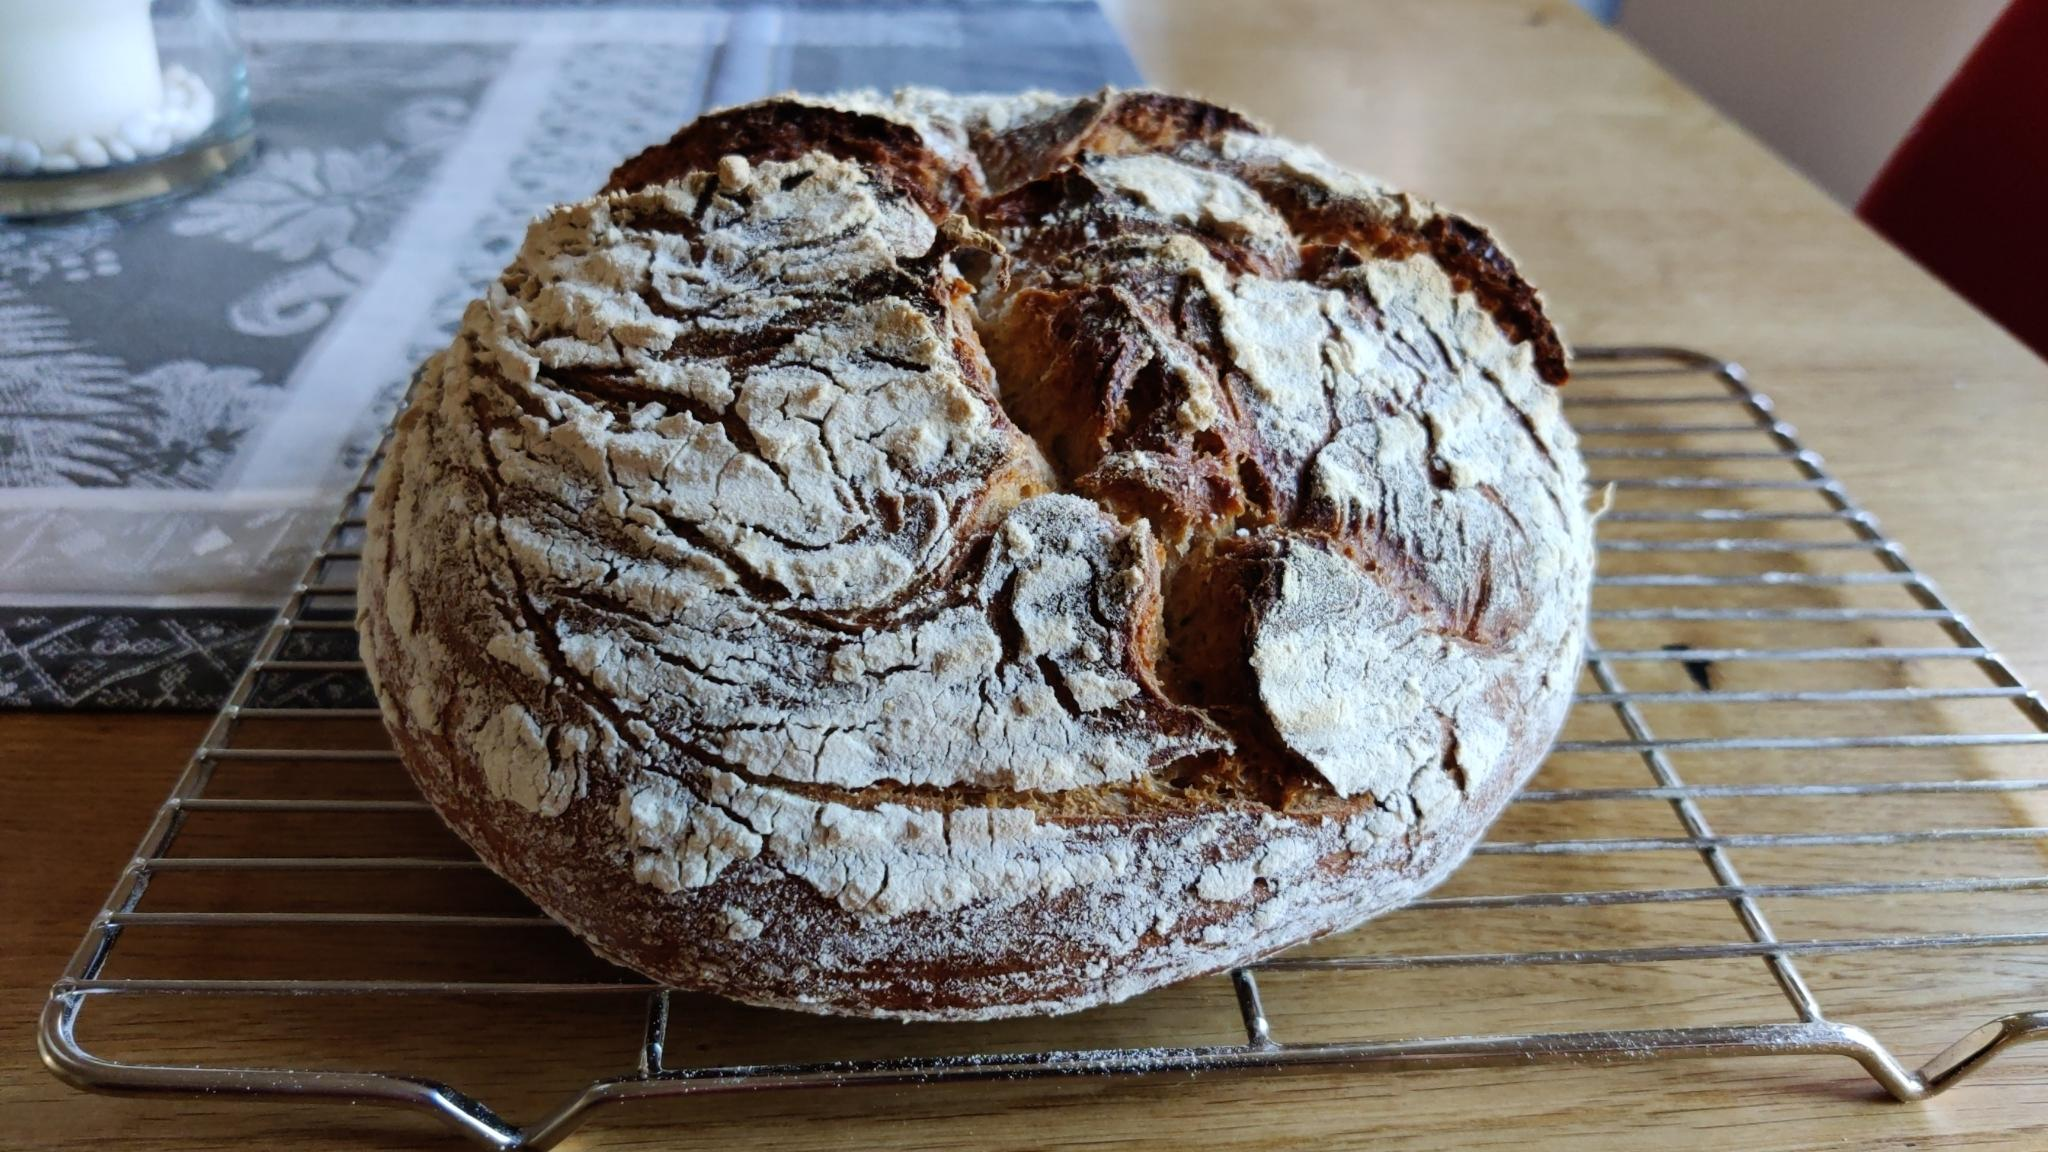
\includegraphics[width=0.7\linewidth]{Bilder/JulesSchwester}
    \caption{Jules Schwester}
    \label{fig:auffrischbrotJulesSchwester}
\end{figure}

\subsection*{Zeitplan}
\begin{tabular}{ r @{ Uhr \phantom{bla} } l}
    \toprule
    \multicolumn{1}{c @{\phantom{ bla }}}{Zeit} & \multicolumn{1}{@{}l}{Aktion} \\ \midrule
    00:00                                       & \Gls{Bruehstueck}             \\
    00:20                                       & \Gls{Fermentolyse}            \\
    01:00                                       & \Gls{Hauptteig}               \\
    01:20                                       & \Gls{Stockgare}               \\
    02:20                                       & \Gls{DehnenUndFalten}         \\
    03:50                                       & \Gls{Formen}                  \\
    04:00                                       & \Gls{Stueckgare}              \\
    05:30                                       & \Gls{Backen}                  \\
    07:10                                       & fertig                        \\ \bottomrule
\end{tabular}
%
%
\subsection*{Alle Zutaten}
\begin{tabular}{r l}
           40 g & Altbrot geröstet                  \\
          120 g & heißer Kaffee                     \\
          150 g & Lievito Madre / Roggen Anstellgut \\
    250 / 225 g & kühles Wasser (LM / Roggen- ASG)  \\
          200 g & Weizenmehl Type 550               \\
          100 g & Weizenmehl Type 1050              \\
          100 g & Roggenvollkornmehl                \\
            5 g & Frischhefe                        \\
           10 g & Rübenkraut                        \\
           12 g & Salz                              \\
           10 g & Rapsöl
\end{tabular}\\




\subsection*{Zubereitung}

\subsubsection*{\Gls{Bruehstueck}}
\begin{tabular}{r l}
    40 g & Altbrot geröstet\\
    120 g & heißer Kaffee\\
\end{tabular}\\

Kurz mischen und für mindestens 30–60 Minuten unbedeckt auf Raumtemperatur abkühlen lassen.

\subsubsection*{\Gls{Fermentolyse}}
\begin{tabular}{r l}
          150 g & Lievito Madre / Roggen Anstellgut \\
    250 / 225 g & kühles Wasser (LM / Roggen- ASG)  \\
          200 g & Weizenmehl Type 550               \\
          100 g & Weizenmehl Type 1050
\end{tabular}\\

Lievito Madre im Wasser auflösen, dann alles kurz, aber gründlich mischen und für 30 Minuten abgedeckt quellen lassen.


\subsubsection*{\GLS{Hauptteig}}
\begin{tabular}{r l}
        + & Fermentolyseteig                     \\
        + & Brühstück abgekühlt                  \\
      5 g & Frischhefe                           \\
     10 g & Rübenkraut                           \\
     12 g & Salz                                 \\
    100 g & Roggenvollkornmehl                   \\
     30 g & Wasser nach Bedarf (\Gls{Bassinage})
\end{tabular}\\

Alle Zutaten (außer Salz + Bassinage) für 8–10 Minuten mit geringer Stufe kneten. Salz hinzufügen, für 3–5 Minuten mit höherer Stufe auskneten. Bei Bedarf noch bis zu 30 g Wasser (Bassinage) mit einkneten.


\subsubsection*{\Gls{Stockgare}}
Den Teig in einer leicht geölten Schüssel oder Teigwanne bei Raumtemperatur abgedeckt etwa 2,5 Stunden bis zur guten Verdopplung reifen lassen, dabei nach 1 dehnen und falten


\subsubsection*{\Gls{Stueckgare}}
Rund wirken und mit dem Schluss nach unten in ein bemehltes Gärkörbchen geben. Abgedeckt für 80 Minuten bei Raumtemperatur (20−22 °C) reifen lassen. 

\subsubsection*{\Gls{Backen}}
Den Backofen rechtzeitig auf 250 °C Ober-/Unterhitze  vorheizen, zusammen mit einem Backstahl oder Backstein.\\
Den Teigling aus dem Gärkörbchen stürzen und einschießen. Sofort schwaden. \\
Nach 10 Minuten den Dampf ablassen und die Temperatur auf 210° C reduzieren. Weitere 40 Minuten backen.

\section[Jule 2.0]{Jule 2.0 \textmd{(siehe \cite{sonjaJule2})}}  \index{Brot!Weizen}\index{Brot!Lievito Madre}\index{Auffrischbrot!Jule 2}

%\begin{figure}[H]
%    \centering
%    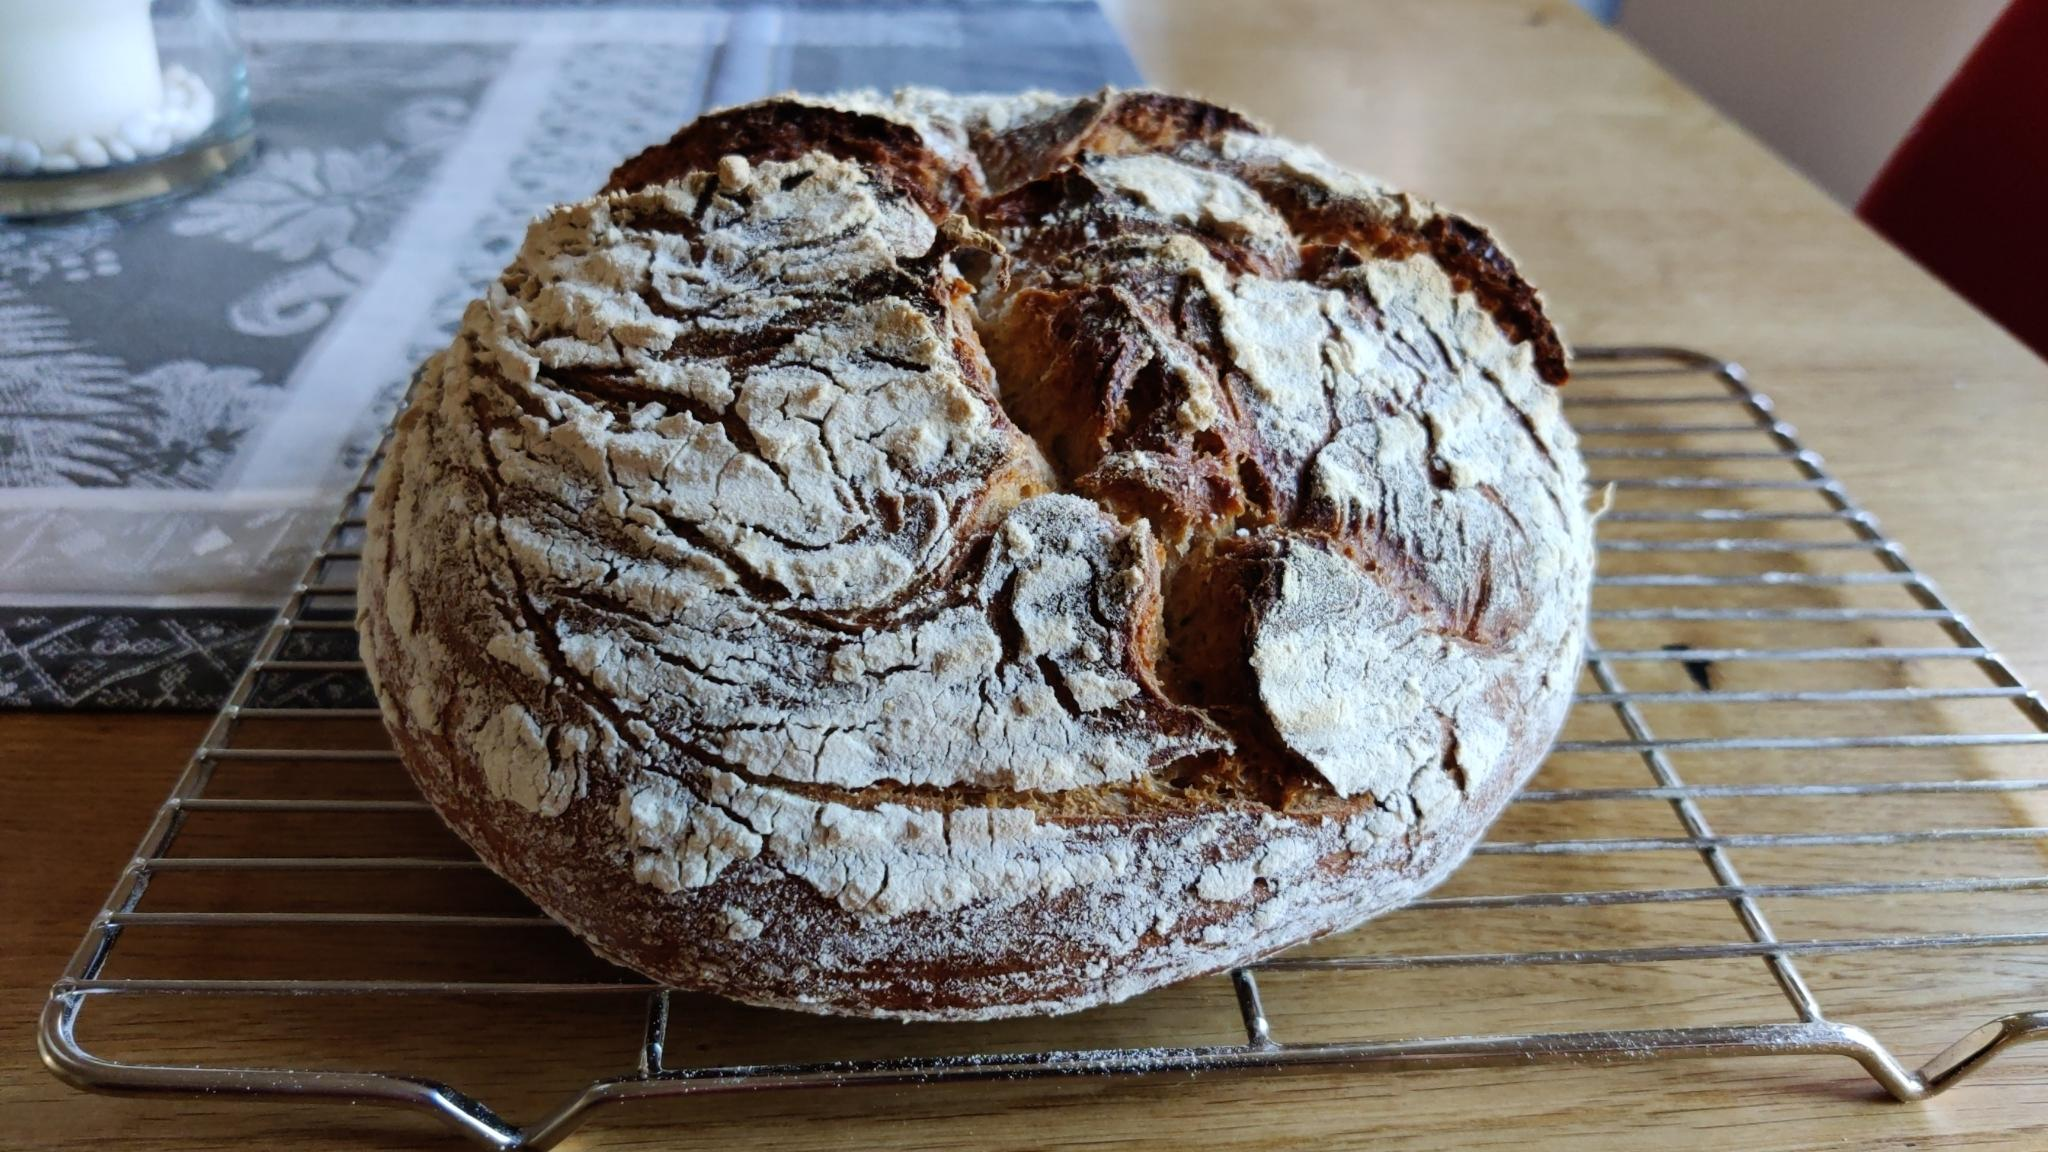
\includegraphics[width=0.7\linewidth]{Bilder/JulesSchwester}
%    \caption{Jules Schwester}
%    \label{fig:auffrischbrotJulesSchwester}
%\end{figure}

\subsection*{Zeitplan}
\begin{tabular}{ r @{ Uhr \phantom{bla} } l}
    \toprule
    \multicolumn{1}{c @{\phantom{ bla }}}{Zeit} & \multicolumn{1}{@{}l}{Aktion}   \\ \midrule
    00:00                                       & \Gls{Bruehstueck}               \\
    00:20                                       & \Gls{Fermentolyse}              \\
    01:00                                       & \Gls{Hauptteig}                 \\
    01:20                                       & \Gls{Stockgare}                 \\
    02:20                                       & \Gls{DehnenUndFalten}           \\
    03:20                                       & \Gls{DehnenUndFalten}           \\
    04:50                                       & \Gls{Formen}                    \\
    05:00                                       & \Gls{Stueckgare} im Kühlschrank \\
    17:30                                       & Vorheizen                       \\
    16:00                                       & \Gls{Backen}                    \\
    16:50                                       & fertig                          \\ \bottomrule
\end{tabular}
%
%
\subsection*{Alle Zutaten}
\begin{tabular}{r l}
           40 g & Altbrot geröstet                  \\
          120 g & heißer Kaffee                     \\
          150 g & Lievito Madre / Roggen Anstellgut \\
    250 / 225 g & kühles Wasser (LM / Roggen- ASG)  \\
          200 g & Weizenmehl Type 550               \\
          100 g & Weizenvolkorn                     \\
           50 g & Roggenvollkorn                    \\
           50 g & Roggen 1150                       \\
            3 g & Frischhefe                        \\
           10 g & Rübenkraut                        \\
           12 g & Salz
\end{tabular}\\


\section{Einfaches Auffrischbrot}  \index{Brot!Weizen}\index{Brot!Lievito Madre}\index{Auffrischbrot! Einfaches}
\begin{figure}[H]
    \centering
    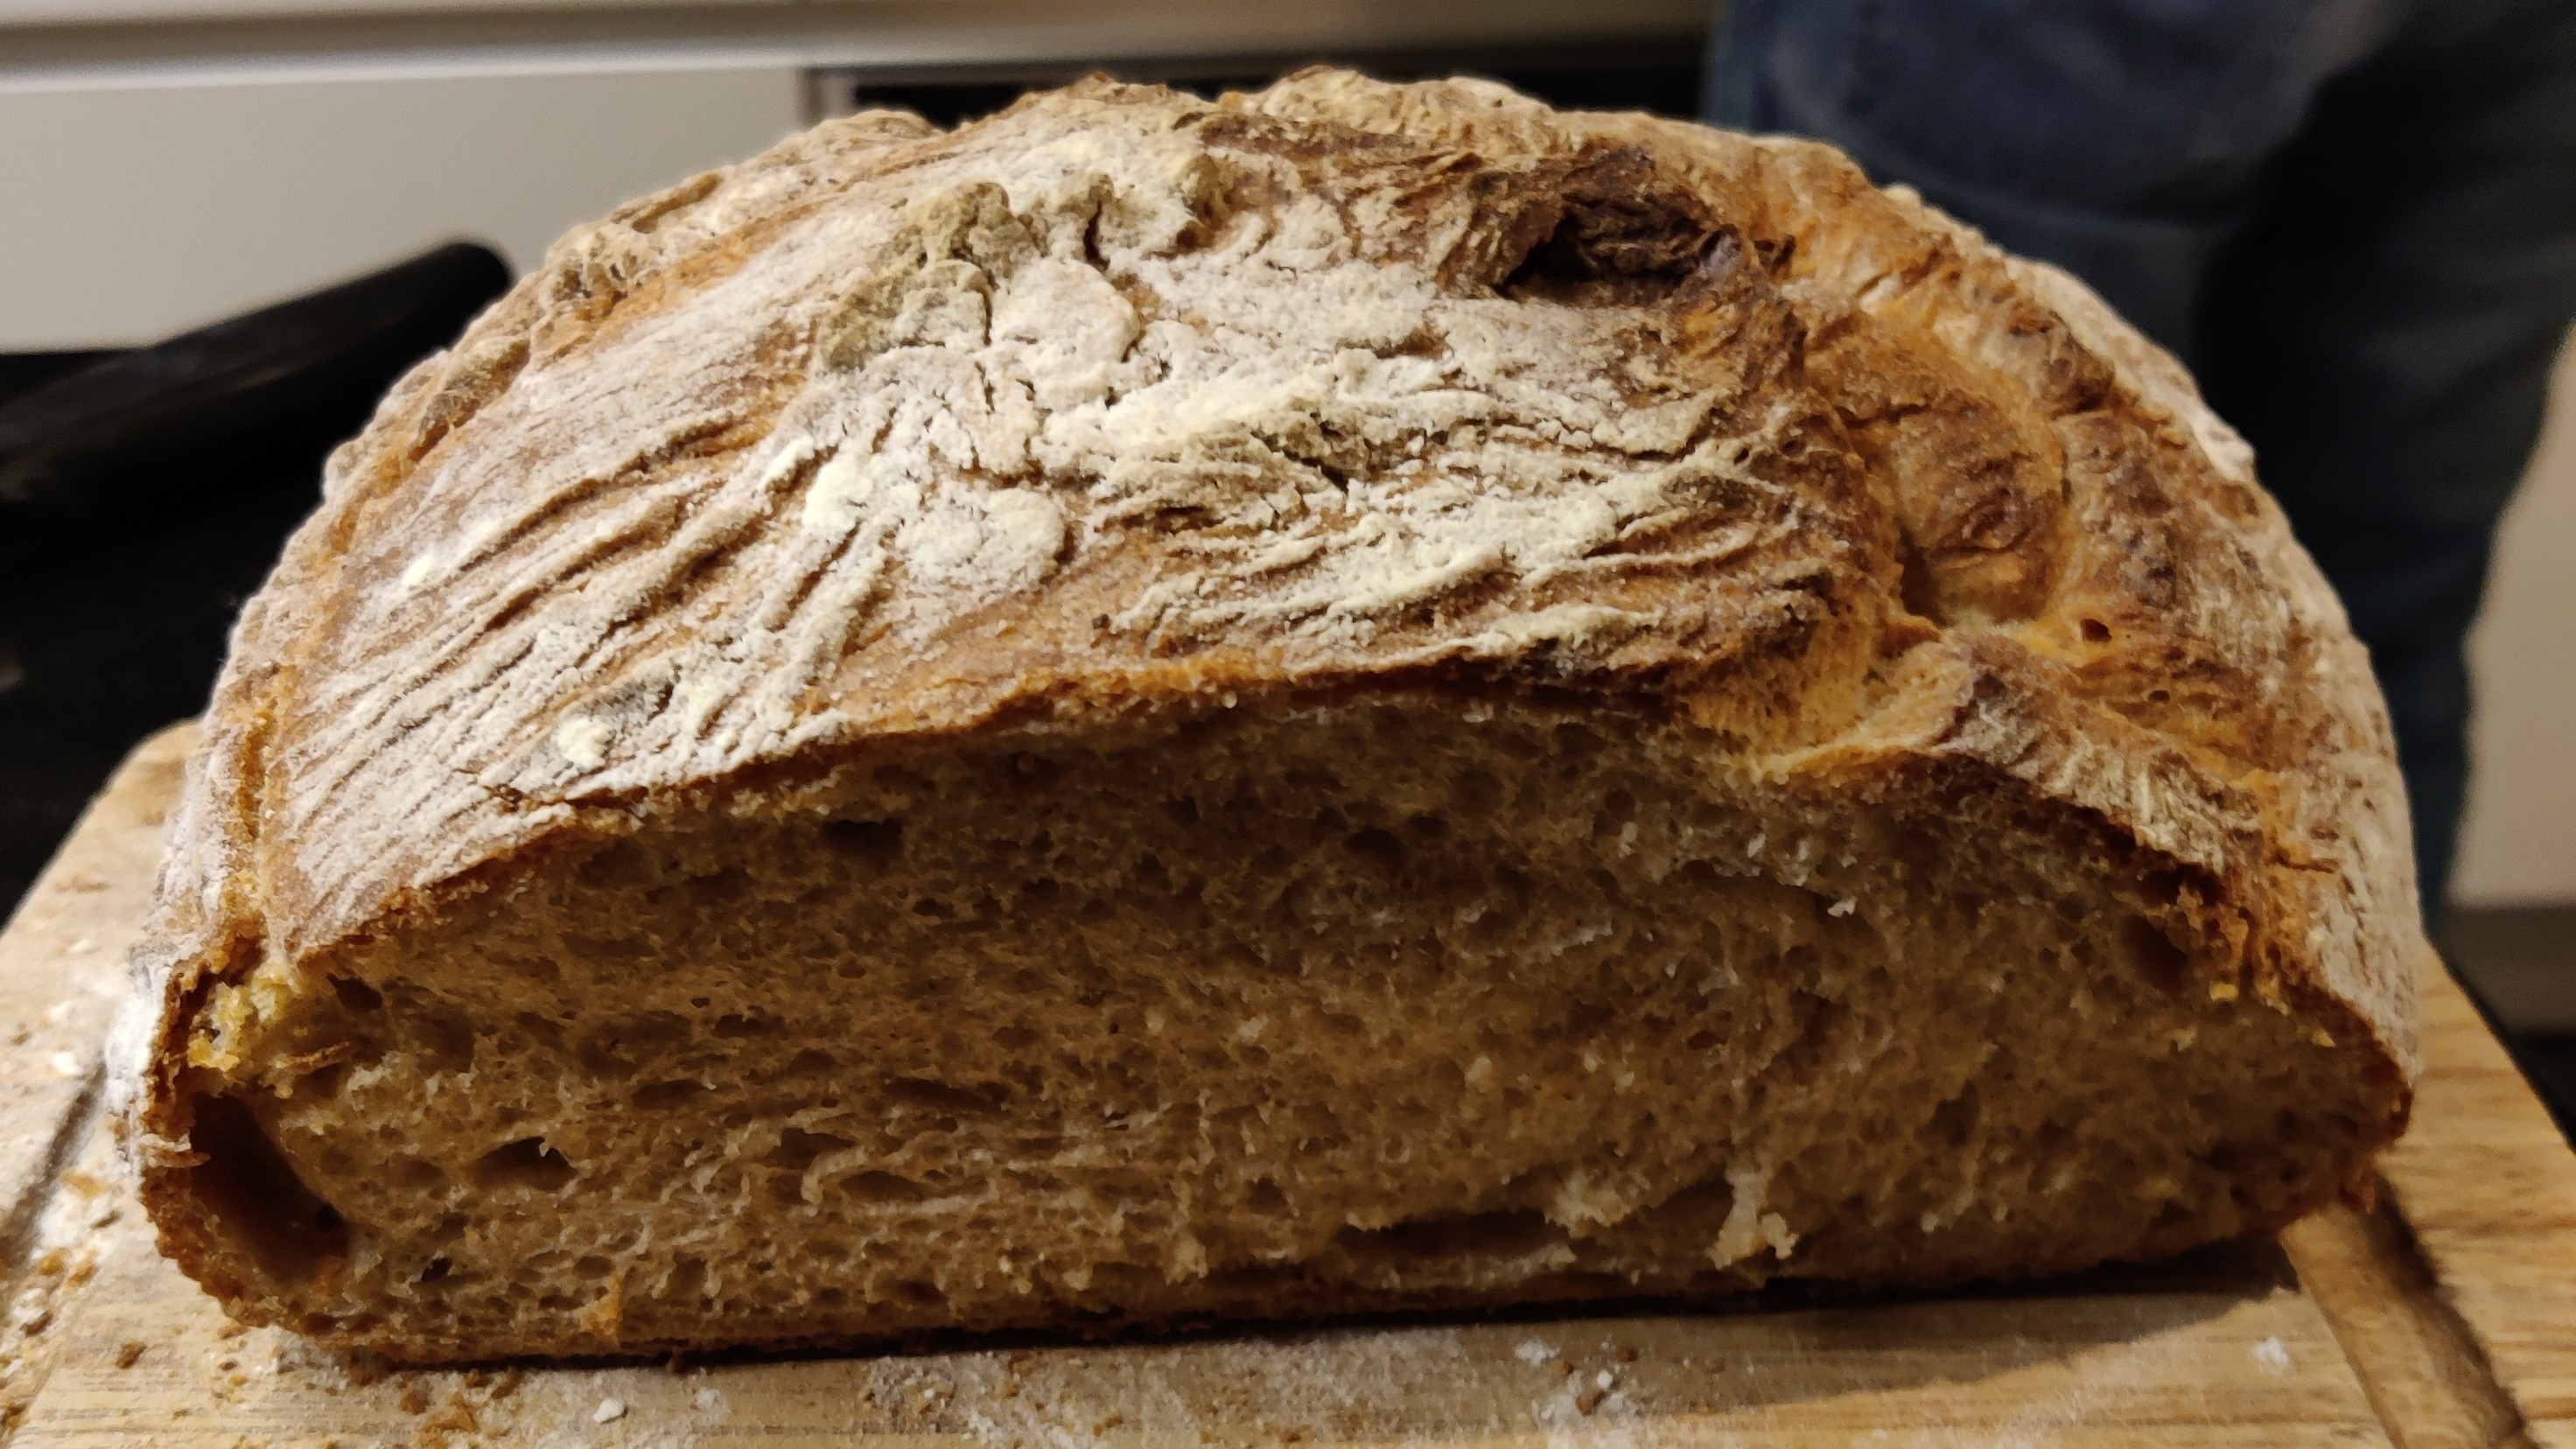
\includegraphics[width=0.7\linewidth]{Bilder/AuffrischbrotEinfach}
    \caption{Auffrischbrot Einfach}
    \label{fig:auffrischbroteinfach}
\end{figure}

\subsection*{Allgemeines}
\begin{tabular}{lrl}
    Gesamtzeit               &              ca. 5.30 & Stunden \\
    Fermentolyseteig mischen &                  0.00 & Uhr     \\
    Hauptteig zubereiten     &                  0.40 & Uhr     \\
    dehnen und falten        &                  1.40 & Uhr     \\
    Stockgare                &                  3.10 & Uhr     \\
    Backofen vorheizen       &                  4.20 & Uhr     \\
    formen + Stückgare       &                  4.50 & Uhr     \\
    backen                   &                  5.40 & Uhr     \\
    siehe                    & \cite[124]{SonjaBauer2021} &
\end{tabular}

\subsection*{Zutaten}

\subsubsection*{\Gls{Fermentolyse}}
\begin{tabular}{r l}
    120 g & Lievito-Madre-Anstellgut (+ 30 g Wasser)\\
    oder 150 g & Roggen ASG \\
    250 g & kühles Wasser\\
    250 g & Weizenmehl Type 550\\
    100 g & Weizenmehl Type 1050\\
    75  g & Vollkornmehl nach Wahl\\
\end{tabular}\\
Lievito Madre im Wasser auflösen, dann alles kurz, aber gründlich mischen und für 30 Minuten abgedeckt quellen lassen.


\subsubsection*{Hauptteig}
\begin{tabular}{r l}
    + & Fermentolyseteig                                      \\
    3 g & Frischhefe          \\
    10 g & Rübenkraut \\
    12 g & Salz                                                  \\
    %    10 g & Butter (oder Olivenöl)                                \\
    40 g & Wasser nach Bedarf (\Gls{Bassinage})                        \\
\end{tabular}\\


\subsection*{Zubereitung}
\begin{enumerate}
    \item [Teig] 
    %        \begin{itemize}
        %        \item Alle Zutaten (außer Salz + Bassinage) für 8–10 Minuten mit geringer Stufe kneten. Salz hinzufügen, für 3–5 Minuten mit höherer Stufe auskneten. Bei Bedarf noch bis zu
        %        40 g Wasser (Bassinage) mit einkneten.
        %\end{itemize}
        Alle Zutaten (außer Salz + Bassinage) für 8–10 Minuten mit geringer Stufe kneten. Salz hinzufügen, für 3–5 Minuten mit höherer Stufe auskneten. 
        
        Bei Bedarf noch bis zu 40 g Wasser (Bassinage) mit einkneten.
        \item [\Gls{Stockgare}]
        Den Teig in einer leicht geölten Schüssel oder Teigwanne bei Raumtemperatur abgedeckt etwa 3-4 Stunden bis zur guten Verdopplung reifen lassen, dabei nach 1 und 2 Stunden schonend dehnen und falten.
        \item [\Gls{Ballengare}]
        Den Teig auf einer bemehlten Arbeitsfäche locker rund wirken und abgedeckt für 20 Minuten mit dem Schluss nach unten entspannen lassen. 
        
        Danach rund wirken und mit dem Schluss nach unten in ein bemehltes Gärkörbchen geben.
        \item [\Gls{Stueckgare}]
        Abgedeckt für 90 Minuten bei Raumtemperatur (20−22 °C) reifen lassen.
        \item [Backen]
        Den Backofen rechtzeitig auf 250 °C Ober-/Unterhitze  vorheizen, zusammen mit einem Backstahl oder Backstein.
        
        Den Teigling aus dem Gärkörbchen stürzen und einschießen. Sofort schwaden. 
        
        Nach 10 Minuten den Dampf ablassen und die Temperatur auf 210° C reduzieren. Weitere 40 Minuten backen.
    \end{enumerate}


\section[Kornkasten]{Kornkasten \textmd{(siehe \cite[182]{SonjaBauer2021})}}  \index{Kastenbrot!Kornkaster}\index{Pollerbrot!Kornkasten}\index{Brot!Kastenbrot} \index{Buttermilch}


%\begin{figure}[H]
%%    \centering
%%    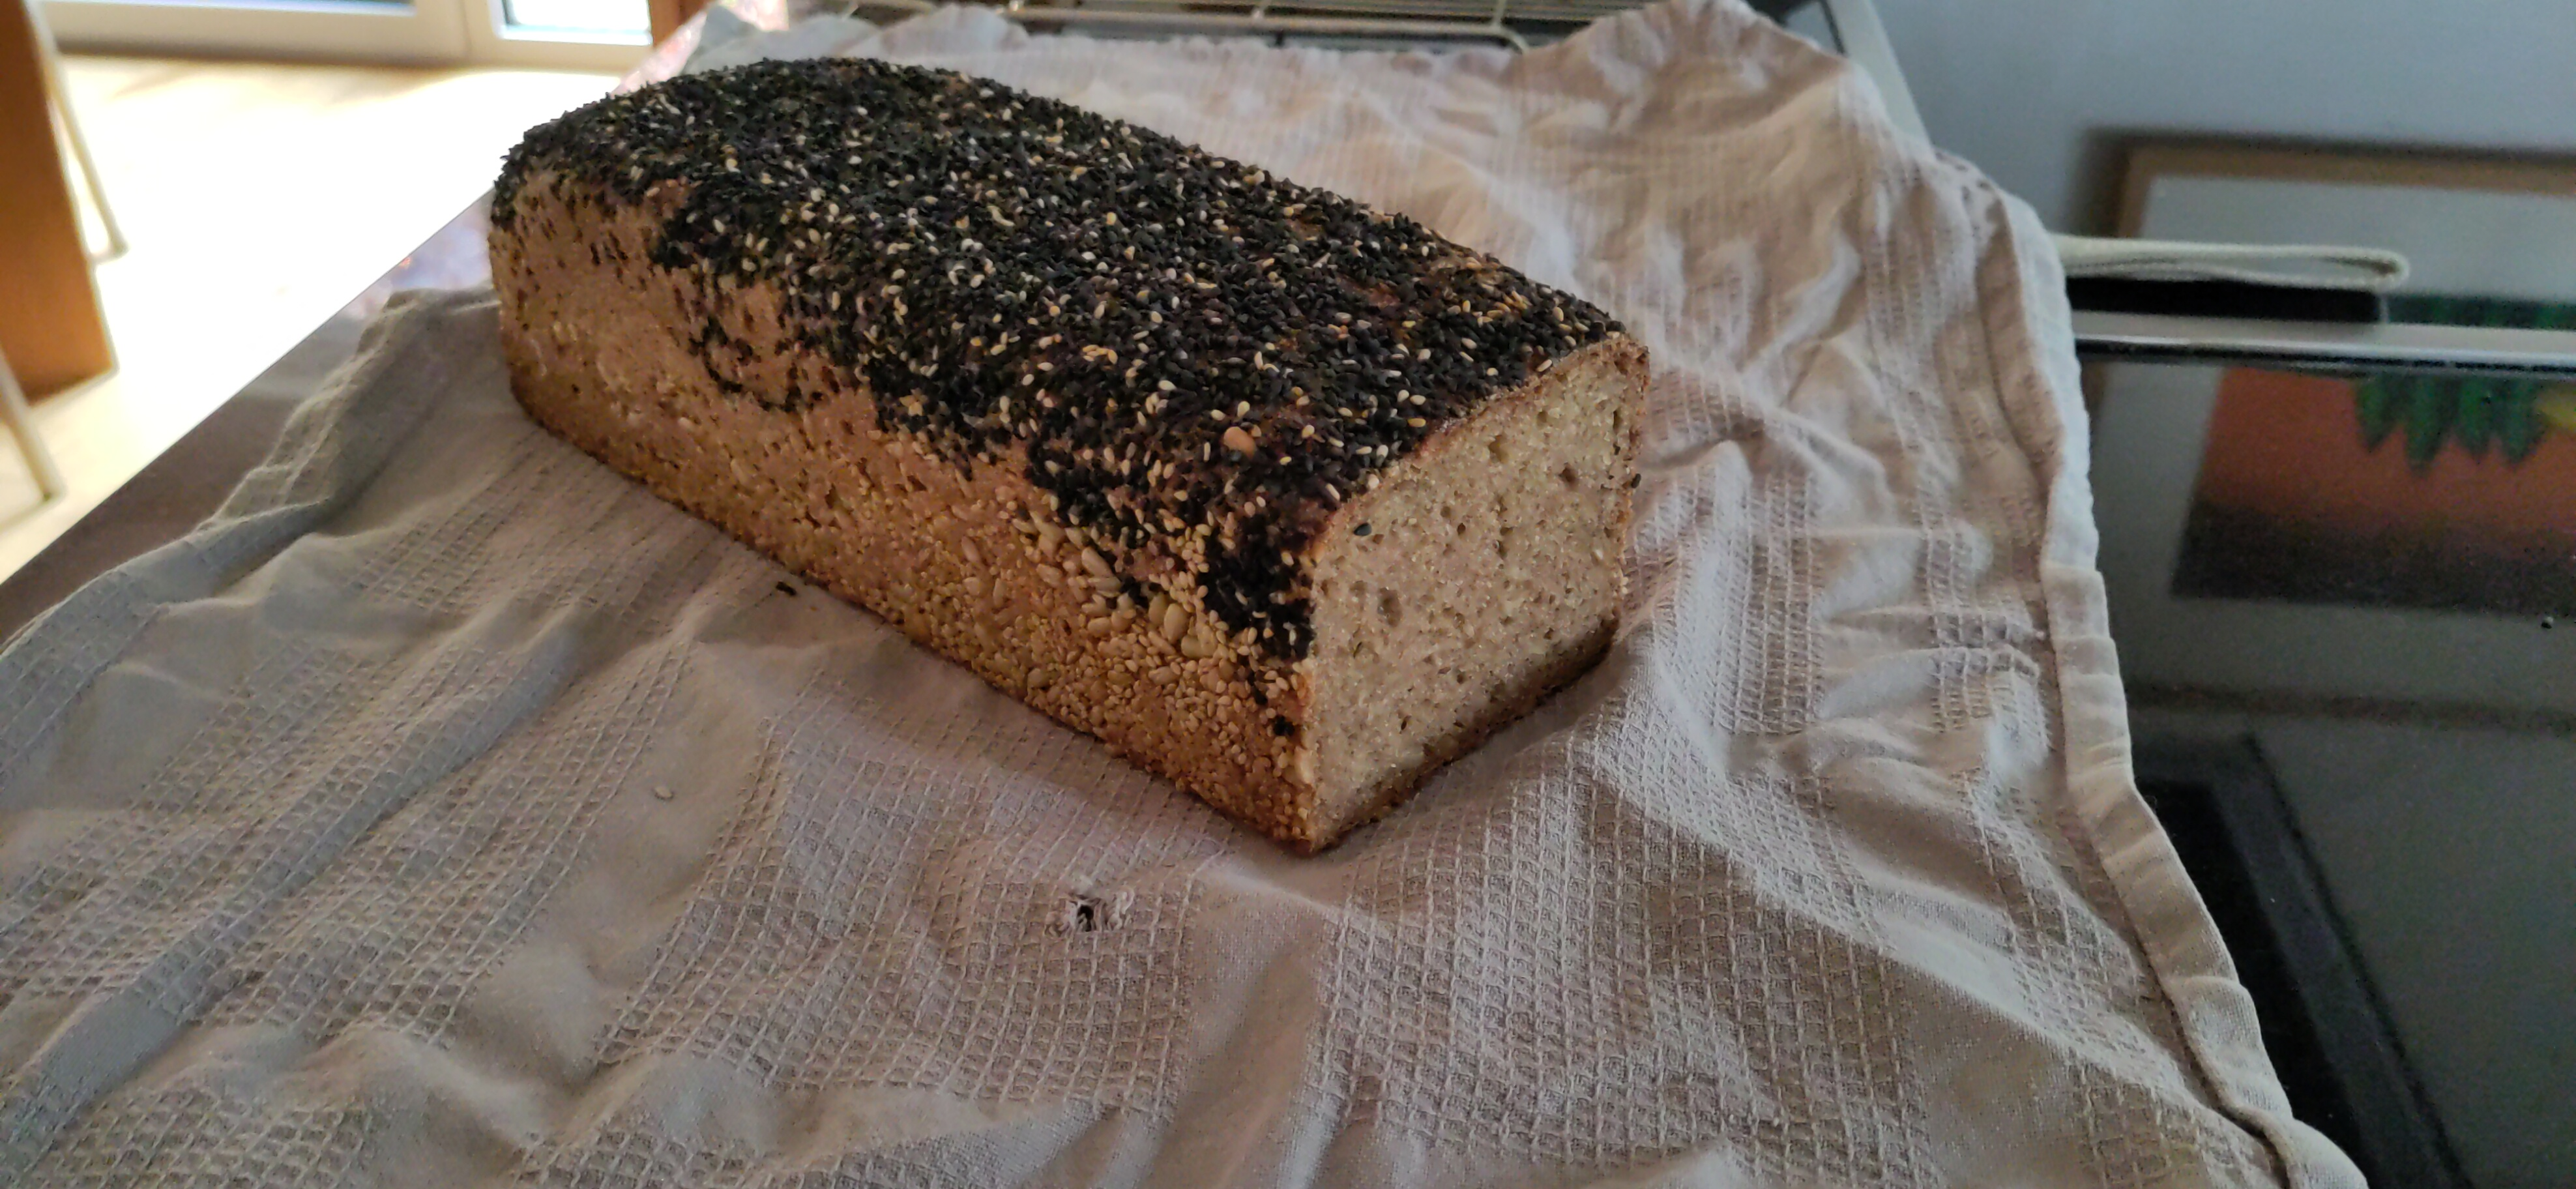
\includegraphics[width=0.7\linewidth]{Bilder/Vollkornprotz}
%%    \caption{Vollkornprotz mit schwarzem Sesam}
%%    \label{fig:vollkornprotz}
%\end{figure}

\subsection*{Zeitplan}
\begin{tabular}{ r @{ Uhr \phantom{bla} } l}
    \toprule
    \multicolumn{1}{c @{\phantom{ bla }}}{Zeit} & \multicolumn{1}{@{}l}{Aktion}   \\ \midrule
    00:00                                       & \Gls{Hauptteig}                 \\
    00:20                                       & \Gls{Stueckgare}     \\
    11:20                                       & Backen                          \\
    11:55                                       & Poller: fertig                  \\ 
    12:20                                       & Kasten: fertig                  \\ 
    \bottomrule
\end{tabular}
%
%
\subsection*{Zutaten}
%\subsubsection*{Alle Zutaten}
\begin{tabular}{r l}
    270  g & Wasser, 35° C         \\
    250  g & Buttermilch, kalt     \\
     25  g & Roggen-ASG (optional) \\
      1  g & Frischhefe            \\
    200  g & Weizenmehl T 1050     \\
    200  g & Roggenvollkornmehl    \\
    100  g & Roggenmehl 1150       \\
    100  g & Dinkelvollkornmehl    \\
      10 g & Rübensirup            \\
     25  g & Leinsamen, geschrotet \\
      14 g & Salz                  \\
      10 g & Rapsöl
\end{tabular}\\

\subsection*{Zubereitung}
\begin{enumerate}
    \item  [\Gls{Hauptteig}]  Wasser und Buttermilch mischen, Anstellgut (ASG) und Frischhefe darin auflösen.\\
    Danach alle Zutaten für den Hauptteig (außer Salz + Öl) hinzufügen und für 8–10     Minuten mit geringer Stufe kneten. In den letzten 2  Minuten Salz und Rapsöl zugeben.\\
    Kastenform oder 3 Weckgläser 0,75() gut einfetten und mit Roggenvollkornmehl oder gemahlenem Altbrot ausstreuen.\\
    Den Teig in Kastenform oder Gläser (Teigeinlage ca. 400 g) einfüllen, die Teigoberfläche mit einem angefeuchteten Teigschaber glattstreichen und mit Roggenvollkornmehl bestreuen. Kastenform bzw. Gläser sind gut zur Hälfte gefüllt.
    \item [\Gls{Stueckgare}] ZIEL: ca. 1 cm unter dem Rand. \\
    Abgedeckt für 10–12 Stunden bei Raumtemperatur zur Gare stellen. Der Teig soll etwa knapp den Rand der Form/Gläser erreichen.
    \item [Backen]  Backofen rechtzeitig mit einem Backstahl oder Backstein auf 230° C Ober-/Unterhitze vorheizen.\\
    Einschießen und wenig schwaden. Für insgesamt etwa 60 Minuten (Kastenbrot) bzw. 35-40 Minuten (Pollerbrote) backen.\\
    Nach 10 Minuten die Temperatur auf 200° C reduzieren. Nach dem Backen aus der Form lösen und nochmal für 10 Minuten bei leicht geöffneter Backofentür zurück in den Ofen geben. 
\end{enumerate}


\chapter{Hefe}
\section{Ciabatta}  \index{Brot!Weizen}\index{Brot!Hefe}\index{Ciabatta}
\subsection*{Allgemeines}
\begin{tabular}{lrl}
    Gesamtzeit          & ca. 17 & Stunden \\
    Vorteig erstellen   &      5 & Minuten \\
    Vorteig ruhen       &     12 & Stunden \\
    Hauptteig erstellen &     10 & Minuten \\
    1. Gehzeit          &      3 & Stunden \\
    Backzeit            &     30 & Minuten
\end{tabular} 
\subsection*{Zutaten}
\begin{tabular}{lrr}
    Hefe               &   2 &  g \\
    Zucker             &   1 & TL \\
    Weizenmehl Tipo 0 &  300 &  g \\
    Hartweizenmehl     &  50 &  g \\
    Wasser             & 225 & ml \\
    Salz               &   1 & TL \\
    Olivenöl           &   4 & EL
\end{tabular} 


\subsection*{Zubereitung}

\begin{enumerate}
    \item Hefe, Zucker, Weizenmehl und 125 ml Wasser glatt rühren und abgedeckt ca. 12 Std. warm ruhen lassen. 
    \item Restliche trockene Zutaten mit dem Vorteig grob mischen. 100 ml
    warmes Wasser mit dem Öl zum Mehl geben und ca. 5 Min. kräftig
    rühren, bis sich der Teig vom Schüsselrand löst. Kein Wasser zugeben. Teig nach der ersten und zweiten Stunde falten \todo{Bilder einfügen} und dann jeweils stehen lassen, Eine weitere Stunde in der Schüssel ruhen lassen.
    
    \item Den Teig auf Backpapier stürzen, zu einem länglichen Laib auseinander ziehen und mit einer Haube abdecken. 1 Std. ruhen lassen.\\
    Den Backofen auf 240° vorheizen, wenn vorhanden mit Backstahl oder Backstein. Das Brot
    mit Wasser besprühen und mit Mehl bestreuen. Etwas Wasser mit in den Ofen und das Brot auf der mittleren Schiene ca.15 Min. backen. Danach die Temperatur auf 210° reduzieren und das Brot in weiteren 15 Min. fertig backen.
    
\end{enumerate}   


\section[Dinkel-Bauernkruste]{Dinkel-Bauernkruste \textmd{(siehe \cite[170]{SonjaBauer2021})}}  \index{Brot!Dinkel-Bauernkruste} \index{Magerquark} \index{Brot!Dinkel}

\subsection*{Zeitplan}
\begin{tabular}{ r @{ Uhr \phantom{bla} } l}
    \toprule
    \multicolumn{1}{c @{\phantom{ bla }}}{Zeit} & \multicolumn{1}{@{}l}{Aktion} \\ \midrule
    00:00                                       & \Gls{Autolyse}                \\
    00:30                                       & \Gls{Hauptteig}               \\
    00:50                                       & \Gls{Stockgare}(20- 22 Grad)  \\
    01:35                                       & \Gls{DehnenUndFalten}         \\
    02:20                                       & \Gls{DehnenUndFalten}         \\
    11:50                                       & \Gls{Formen}                  \\
    12:00                                       & \Gls{Stueckgare}              \\
    13:00                                       & Vorheizen                     \\
    13:30                                       & \Gls{Backen}                  \\
    14:15                                       & fertig                        \\ \bottomrule
\end{tabular}

\subsection*{Alle Zutaten}
\begin{tabular}{r l}
    280 g & Wasser, kühl       \\
    0,8 g & Acerola-Pulver     \\
    100 g & Magerquark, kalt   \\
    350 g & Dinkelmehl  630    \\
      5 g & Flohsamenschalen   \\
    150 g & Dinkelvollkornmehl \\
      1 g & Hefe               \\
     10 g & Honig              \\
     12 g & Salz               \\
     10 g & Butter             \\
     20 g & Bassinage
\end{tabular}\\

\subsection*{Zubereitung}
    \subsubsection*{\GLS{Autolyse}} 
    \begin{tabular}{r l}
        280 g & Wasser, kühl       \\
        0,8 g & Acerola-Pulver     \\
        100 g & Magerquark, kalt   \\
        350 g & Dinkelmehl  630    \\
          5 g & Flohsamenschalen   \\
        150 g & Dinkelvollkornmehl
    \end{tabular} 
    
         Acerola in dem Wasser auflösen. Danach alles kurz,aber gründlich mischen und für 30 Minuten abgedeckt quellen lassen.
    
    \subsubsection*{\Gls{Hauptteig}}  
    \begin{tabular}{r l}
           + & Autolyse  \\
         1 g & Hefe      \\
        10 g & Honig     \\
        12 g & Salz      \\
        10 g & Butter    \\
        20 g & Bassinage
    \end{tabular}
    
    Alle Zutaten (außer Salz + Butter + Bassinage) für 8–10 Minuten mit geringer Stufe kneten. Salz und Butter zugeben, für 1–2 Minuten mit höherer Stufe auskneten. Dabei bei Bedarf bis zu 20 g Wasser (Bassinage) mit einkneten.
    
    \subsubsection*{\Gls{Stockgare}}
    Abgedeckt für 10–12 Stunden bei Raumtemperatur zur Gare stellen. Nach 45 und 90 Minuten dehnen und falten.
    
    \subsubsection*{\GLS{Formen}}
    Auf der bemehlten Arbeitsfläche schonend rund wirken und mit dem Schluss nach unten in ein bemehltes Gärkörbchen geben.
    
    \subsubsection*{\Gls{Stueckgare}} 
    Abgedeckt für 10–12 Stunden bei warmer Raumtemperatur (22–24° C) zur Gare stellen. Der Teig soll etwa knapp den Rand der Form erreichen.
    \subsubsection*{\Gls{Backen}}
    Backofen rechtzeitig auf 250° C Ober–/Unterhitze vorheizen.\\
    Teigling aus dem Gärkörbchen stürzen und einschießen. Sofort schwaden und für insgesamt 40–50
    Minuten backen. Nach 10 Minuten den Dampf ablassen und die Temperatur auf 210° C reduzieren.
    

















 
 
 

 











\glsaddall

\newglossaryentry{Autolyse}{
    name={Autolyse},
    description={Siehe auch Nullteig. Die Autolyse bzw. der Autolyseteig wird vor der eigentlichen Teigzubereitung aus Mehl und Wasser oder an-
        deren Schüttflüssigkeiten gemischt und ruht meist abgedeckt für 20 bis 60 Minuten – manchmal auch bis zu 2 Stunden oder sogar über Nacht im Kühlschrank. Dabei verquellen Wasser, Stärke und Eiweißbestandteile aus dem Mehl. Während der Ruhezeit verkettet sich das Klebereiweiß (Gluten), und es bilden sich Glutenstränge (Teigstruktur). Dadurch kann die Knetzeit deutlich reduziert und einer zu starken Erwärmung beim Knetprozess vorgebeugt werden.
}}

\newglossaryentry{Backen}{
        name={Backen},
        description={Das Backen löst im Teig komplexe physikalische und chemische Prozesse aus. Je nach der Temperatur an der Teiglingsoberfläche und im Inneren des Teiglings beginnen unterschiedliche Vorgänge, bei denen sich Krume und Kruste bilden. Die jeweiligen Prozesse laufen nicht gleichmäßig im gesamten Teigling ab, sondern wandern von außen nach innen. Während zum Beispiel in den Randbereichen des Brotes schon alle Mikroorganismen durch die Hitze abgetötet sind, können sie im Inneren weiter für Ofentrieb sorgen.\\
        Quelle: \cite{PloetzblogLexikon2023}
        }}

\newglossaryentry{Ballengare}{
    name={Ballengare},
    description={Die sogenannte Ballengare oder Zwischengare dient als kurze Entspannungsphase für die Kleberstränge. Der Teig wird dabei zunächst locker vorgeformt (meinst rund) und ruht dann abgedeckt (z. B. mit einem Geschirrtuch) zwischen 5–20 Minuten. Dadurch lassen sich manche Teige besser formen oder reißen beim späteren Formen nicht. Anschließend folgt die endgültige Formgebung des Teiges.
}}

\newglossaryentry{Bassinage}{
    name={Bassinage},
    description={Verfahren, ein Teil des Schüttwassers im Knetprozess von Weizenteigen erst am Ende der Knetzeit schluckweise zuzugeben, wenn man bereits eine gute Kleberentwicklung erreicht hat. Dieses Verfahren wird insbesondere bei Teigen mit einem hohen Wassergehalt = hohe Teigausbeute genutzt.
}}

\newglossaryentry{Bruehstueck}{
    name={Brühstück},
    description={Das Brühstück gehört zur Gruppe der Nullteige innerhalb der Vorstufen. Es dient der Verquellung gröberer Brotbestandteile (z.B. Körner, Saaten, Schrote), um den Kaueindruck und die Frischhaltung zu verbessern (siehe auch Quellstück und Kochstück).\newline       
    Für ein Brühstück werden die festen Bestandteile im Verhältnis von ca. 1 : 1 bis 1 : 3 mit kochendem Wasser vermischt und mindestens 2-6 Stunden quellen gelassen. Eine noch optimalere und im Hobbybäckerbetrieb zeitlich passendere Variante ist das Verquellen über 8-12 Stunden bei 6-8°C im Kühlschrank (nachdem das Brühstück ausgekühlt ist). Um enzymatischen Abbau und Fremdgärung zu verhindern, kann die Salzmenge des Hauptteiges mit in das Brühstück eingerührt werden.\newline
    Würden die groben Bestandteile nicht verquollen, würde der Wassergehalt im Teig sinken und der Teig durch Nachquellung zunehmend fester und trockener werden. Üblicherweise sollte die im Brühstück zu verquellende Schrotmenge nicht mehr als 30-50\% der Gesamtmenge der Getreideerzeugnisse ausmachen, da durch das heiße Wasser bereits Stärke verkleistert und dem enzymatischen Abbau stärker ausgesetzt ist.\newline 
    Neben Schrot kann z.B. auch getrocknetes und gemahlenes Brot überbrüht werden. Dieses Altbrot bindet etwa die dreifache Menge seines Eigengewichtes an Wasser.\newline
    Quelle: \cite{PloetzblogLexikon2023} 
}}

\newglossaryentry{DehnenUndFalten}{
        name={Dehnen und Falten},
        description={Das Dehnen und Falten von Teig ist ein Vorgang, bei dem weizendominierten Teigen durch mehrfache Dehnung und Faltung mehr Struktur verliehen wird. Das Klebergerüst wird damit schonend entwickelt. Das Gashaltevermögen steigt. Außerdem dient es der Entgasung und Sauerstoffzufuhr, der Homogenisierung der Teigtemperatur und damit der Unterstützung der mikrobiellen Aktivität.\newline
        Quelle: \cite{PloetzblogLexikon2023} 
        }}

\newglossaryentry{Fermentolyse}{
    name={Fermentolyse},
    description={Das Pendant zur \Gls{Autolyse}. Im Gegensatz dazu ist aber bereits ein Triebmittel (Sauer teig/Vor teig) enthalten. Dadurch verkürzt sich das Vorquellen deutlich auf maximal 20 bis 40 Minuten. Dabei verquellen Wasser, Stärke und Eiweißbestandteile aus dem Mehl. Während der Ruhezeit verkettet sich das Klebereiweiß (Gluten), und es bilden sich Glutenstränge (Teigstruktur). Dadurch kann die Knetzeit deutlich reduziert und einer zu starken Erwärmung beim Knetprozess vorgebeugt werden.
}}


\newglossaryentry{Formen}{
    name={Formen},
    description={Nach der Stockgare und vor der nachfolgenden Stückgare wird der Teig geformt. Der Teig kann rund geformt werden (rundwirken), länglich (langwirken) oder auch in allerlei andere Formen gebracht werden. Dies erfolgt überwiegend auf der bemehlten und selten auf der mit Wasser benetzten Arbeitsfläche.\\
    Ziel ist in aller Regel dabei, dass der Teig nicht nur in Form gebracht wird, sondern an der Teigoberfläche auch eine gewisse Spannung aufbaut. Der Teig sollte dabei aber nur so weit gestrafft werden, dass er nicht reißt.       
}}


\newglossaryentry{Hauptteig}{
        name={Hauptteig},
        description={Der Teig, in dem alle Bestandteile des Brotes enthalten sind.
        }}

\newglossaryentry{LievitoMadre}{
    name={Lievito Madre},
    description={Lievito Madre ist Italiens Antwort auf den traditionellen Sauerteig. Mit seiner festen Konsistenz und dem milden Geschmack ist er ein unverzichtbares Element in der italienischen Brotkultur. Ein Lievito Madre ist ein spezieller italienischer Weizensauerteig, der fest geführt wird. Er ist mild und triebstark und auch für süße Backwaren geeignet.         
}}

\newglossaryentry{Quellstueck}{
    name={Quellstück},
    description={Ein Quellstück ist eine wichtige Komponente beim Brot backen, insbesondere wenn das Rezept gröbere oder trockenere Zutaten wie Altbrot, Samen, Schrot oder Trockenfrüchte enthält. Dieser sogenannte Nullteig oder Vorstufe hilft dabei, diese trockenen Zutaten vorzuquellen, indem sie in einem Verhältnis von etwa 1:1 bis 1:2 mit kühlem oder lauwarmem Wasser übergossen werden.
}}

\newglossaryentry{Sauerteig}{
        name={Sauerteig},
        description={In einem Sauerteig entwickeln sich homofermentative (milchsäurebildende) und
        heterofermentative (essigsäurebildende) Milchsäurebakterien (letztere werden oftmals fälschlicherweise als Essigsäurebakterien bezeichnet), außerdem Hefen. 
        Die heterofermentativen Bakterien erzeugen außerdem Kohlenstoffdioxid, das gemeinsam mit dem Kohlenstoffdioxid der alkoholischen Hefegärung das Gärgas bildet und für den Trieb sorgt.
        }}

\newglossaryentry{Stueckgare}{
    name={Stückgare},
    description={
        Die letzte Reifezeit des geformten Teiges vor dem Backen. Die Stückgare er folgt entweder mit Schluss nach oben oder nach unten in einem Gärkörbchen, Bäckerleinen oder in einer Backform.
        Die Stückgare kann je nach Rezept bei Raumtemperatur, an einem
        warmen Ort oder auch kalt erfolgen.
}}
\newglossaryentry{Stockgare}{
    name={Stockgare},
    description={Zeit die man dem Teig nach dem Kneten lässt um sich zu entwickeln. Weiche Weizenteige werden oft während der Stockgare gedehnt und gefaltet um die Teigstruktur zu verbessern. Zur Stockgare wird der Teig in einer Schüssel oder Wanne luftdicht abgedeckt damit er nicht austrocknet
}}

\newglossaryentry{Vorheizen}{
        name={Vorheizen},
        description={Der Ofen sollte bei Ober/Unterhitze ausreichend lange vorgeheizt werden, um das perfekte Brot zu backen. Umluft eignet sich weniger gut, da diese Einstellung die Oberfläche des Brotes zu schnell austrocknen würde.
        }}

\newglossaryentry{Zwischengare}{
    name={Zwischengare},
    description={Die Zwischengare ist eine sehr kurze (ca. 5 – 30 Minuten) Ruhephase zwischen Arbeitsvorgängen. Häufig wird die Zwischengare genutzt, um die Kleberstränge rundgewirkter Teiglinge kurz entspannen zu lassen. Andernfalls würde die Teigoberfläche beim weiteren Wirken reißen. \cite{PloetzblogLexikon2023}
}}




%\newglossaryentry{ }{
    %    name={},
    %    description={
        %}}


%
%
%
%Beschreibung:
%Das Brühstück gehört zur Gruppe der Nullteige innerhalb der Vorstufen. Es dient der Verquellung gröberer Brotbestandteile (z.B. Körner, Saaten, Schrote), um den Kaueindruck und die Frischhaltung zu verbessern (siehe auch Quellstück und Kochstück).
%
%Für ein Brühstück werden die festen Bestandteile im Verhältnis von ca. 1 : 1 bis 1 : 3 mit kochendem Wasser vermischt und mindestens 2-6 Stunden quellen gelassen. Eine noch optimalere und im Hobbybäckerbetrieb zeitlich passendere Variante ist das Verquellen über 8-12 Stunden bei 6-8°C im Kühlschrank (nachdem das Brühstück ausgekühlt ist). Um enzymatischen Abbau und Fremdgärung zu verhindern, kann die Salzmenge des Hauptteiges mit in das Brühstück eingerührt werden.
%
%Würden die groben Bestandteile nicht verquollen, würde der Wassergehalt im Teig sinken und der Teig durch Nachquellung zunehmend fester und trockener werden. Üblicherweise sollte die im Brühstück zu verquellende Schrotmenge nicht mehr als 30-50% der Gesamtmenge der Getreideerzeugnisse ausmachen, da durch das heiße Wasser bereits Stärke verkleistert und dem enzymatischen Abbau stärker ausgesetzt ist.
%
%Neben Schrot kann z.B. auch getrocknetes und gemahlenes Brot überbrüht werden. Dieses Altbrot bindet etwa die dreifache Menge seines Eigengewichtes an Wasser.
%
%Quellen:
%Steffen, Lutz Geißler
%/home/thomas/Sandbox/Privat/Privat/Text/Kochbuch/Glossar.tex
%A
%
%Anstellgut (ASG) : Als Anstellgut bezeichnet man die Sauerteigkultur, die man zum Ansetzen eines neuen Sauerteigs benutzt. Ich lagere meine Sauerteigkultur = Anstellgut im Marmeladenglas im Kühlschrank für bis zu 3 Wochen. Dann muss die Kultur aufgefrischt werden, d.h. 50 g Mehl/50 g Wasser/10 g alte Kultur = Anstellgut für ca. 16-20 h von 30° C auf Raumtemperatur fallend stehen lassen, danach im Kühlschrank lagern. Grundsätzlich kann man einen Sauerteig durch Auffrischen mit einer anderen Mehlsorte umzüchten, also z.B. von Roggen- nach Weizensauerteig. Teilweise wird das Anstellgut auch als Starter bezeichnet.
%
%Auffrischen: Als Auffrischen bezeichnet der Bäcker das Füttern der Sauerteigkultur mit frischem Mehl und Wasser, damit die Mikroorganismen frische Nahrung bekommen und sich wieder vermehren können. Übliche Verhältnisse zum Auffrischen von weichem Sauerteig ist ein Verhältnis 1:5:5 oder 1:10:10 von Anstellgut/Wasser/Mehl.
%
%Autolyse: Als Autolyse bezeichnet man das Quellenlassen von Mehl mit Wasser für 20-60 min ohne die Zugabe von Salz. Dabei quellen die Stärke und die Eiweiße im Mehl auf, was die Backeigenschaften verbessert und das Kneten beschleunigt.
%B
%
%Bassinage: Verfahren, ein Teil des Schüttwassers im Knetprozess von Weizenteigen erst am Ende der Knetzeit schluckweise zuzugeben, wenn man bereits eine gute Kleberentwicklung erreicht hat. Dieses Verfahren wird insbesondere bei Teigen mit einem hohen Wassergehalt = hohe Teigausbeute genutzt.
%D
%
%Dehnen und Falten (oft auch  “stretch and fold” oder s+f genannt)
%Weiche Weizenteige können über das wiederholte dehnen und falten schonend eine gute Struktur bekommen. Dazu wird, vorzugsweise  in einer geölten Wanne oder Schüssel, mit den feuchten Händen eine Seite des Teigs nach oben gezogen und dann über den Teig gefaltet , diesen Vorgang wiederholt man  auf den anderen 3 Seiten. Nach 20 -30 min kann man dann eine weitere Runde starten. Man merkt dabei, dass der Teig wesentlich mehr Struktur bekommt und straffer wird.
%E
%
%Einschießer/Einschießen
%Als Einschießen bezeichnet man den Vorgang den Teigling  mit einem Schieber oder Einschießer in den  Ofen zu bringen. Als Hobbybäcker benutzt man dafür meist ein passendes Brett und verwendet als Trennmittel Gries, feinen Schrot oder einfach Backpapier.
%
%Entgasen/Ausstoßen
%Wenn ein Teig nach der Stockgare gut aufgegangen ist, drückt man ihn mit der flachen Hand oder der Faust auf der Arbeitsfläche platt und sorgt damit dafür, dass sich große Gärblasen verteilen und auch ein Austausch von Kohlendioxid gegen Luftsauerstoff stattfindet was die weitere Entwicklung der Hefen fördert.
%F
%
%Fenstertest: Der Fenstertest dient zur Beurteilung der Kleberentwicklung eines weizenlastigen Teiges. Dazu zieht man den gekneteten Teig zwischen den feuchten Fingern so dünn, dass Licht durchscheint. Reißt der Teig davor ist er noch nicht ausreichend geknetet.
%
%Fingertest: Mit dem Fingertest prüft man die Gare eines Teiglings während der Stückgare: Dazu drückt man leicht mit dem Finger auf den Teigling und kann mit etwas Erfahrung die folgenden Garezustände unterscheiden:
%
%Untergare: Abdruck springt schnell und komplett wieder zurück
%knappe Gare: Abdruck geht langsam und fast  komplett zurück
%Volle Gare: Abdruck geht nur noch wenig zurück es bleibt eine leichte Delle
%Übergare: Abdruck bleibt unverändert oder Teigling fällt sogar zusammen
%
%G
%
%Glutenentwicklung: (Kleberentwicklung) Beim Kneten des Teigs vernetzt sich das Gluten (Kleber) immer stärker, um ein großvolumiges Brot zu erhalten ist eine gute Glutenentwicklung notwendig, diese kann durch den sog. Fenstertest überprüft werden.
%H
%
%Hefe: Hefe ist neben Sauerteig das wichtigste Triebmittel in allen Brotteigen. Man kann Trocken- oder Frischhefe einsetzen. Alle Angaben in meinen Rezepten beziehen sich auf Frischhefe.
%Umrechnungsregel: Trockenhefe in Frischhefe: 1 g Trockenhefe entspricht 3 g Frischhefe.
%Als Hilfe für das Portionieren kleiner Hefemengen gibt es eine sog. Hefeschablone, auch käuflich bei der Draxmühle zu erwerben.
%L
%
%Lievito Madre (LM): LM ist ein sehr milder und triebstarker Weizensauerteig italienischem Ursprungs. Er wird oft für helle Brote, Brötchen und auch für Pannetone verwendet. LM wird recht fest, mit einer Teigausbeute von 150 geführt, d.h. auf 100 g Mehl 50 g Wasser und führt zu einem starken Ofentrieb.
%
%Aufgefrischt wird LM normalerweise so: 1 Teil alter LM, 1 Teil Weizenmehl, 0,5 Teile Wasser (35 -40°C) zu einem festen Teig verkneten, kreuzwesie einschneiden und abgedeckt 4 h bei 30°C gehen lassen.  Dabei soltle er sich mindestens verdoppeln. Dann ist er zum Backen bereit. Nicht vergessen etwas LM abzuzweigen und als “Starterkultur” im Kühlschrank aufbewahren.
%
%Langwirken: Als Langwirken bezeichnet man das Formen eines länglichen Brotlaibs. Man startet immer in dem man den Teig rundwirkt (siehe unten) und ihn. dann nach kurzer Entspannungspause in eine längliche Form bringt. Dafür gibt es diverse Techniken, z.B. hier im Video erklärt.
%P
%
%Poolish: Flüssiger Weizenvortieg mit Hefe: Weizenmehl wird 1:1 mit Wasser gemischt und mit wenig Hefe  (0,2-0,3 %) versetzt und 12-14 h bei Raumtemperatur oder im Kühlschrank stehen lassen.
%R
%
%Rundschleifen: Nennt der Bäcker den Vorgang zum Formen runder Brötchen, es gibt diverse Filmchen dazu bei YouTube
%
%Rundwirken:  So nennet man den Vorgang aus einem Teig einen runden Laib zu formen und dabei im Teig Spannung aufzubauen.  Am besten schaut mich das in einem Video auf YouTube an
%S
%
%Schluß: Die Seite eines Teiglings auf der der Teig eingefaltet wird um Spannung im Teigling zu erzeugen, wird als Schluß bezeichnet. Backt man ein Brot oder Brötchen mit dem Schluß nach oben, reisst die Oberfläche rustikal auf und es muss nicht eingeschnitten werden.
%
%Schwaden: Bäckerdeutsch für  Dampf, der im Ofen erzeugt wird, dies ist insbesondere in der ersten Backphase wichtig damit, ein guter Ofentrieb und eine schöne rösche Kruste erhalten wird. Später wird der Dampf meist abgelassen, damit die Kruste kross wird.
%
%Stippen: So nennt der Bäcker den Vorgang in die Oberfläche eines Teiglinge vor dem Backen kleine Löcher zu machen, dafür gibt es spezielle Stippwalzen/Stipproller/Teigigel oder man behilft sich z.B. mit einem Schaschlikspieß oder ähnlichem. Die dient dazu bei einem fast vollgaren Brot das aufreißen der Kruste zu verhindern.
%
%t.
%
%Stückgare: Zeit in dem sich der Teigling nach dem Formen entwickelt und die richtige Gare vor dem Backen erreicht. Wichtig ist es die Teiglinge mit einem Küchentuch und Folie abzudecken, damit sie nicht austrocknen.
%T
%
%Teigausbeute (TA): Die Teigausbeute gibt das Verhältnis von Mehl zu Flüssigkeit im Teig an, eine hohe Teigausbeute bedeutet, dass viel Flüssigkeit im Teig vorhanden ist. Berechnet wird sie folgendermaßen: Teigausbeute = Flüssigkeitsmenge/Mehlmenge*100+100,
%also z.B. 650g  Wasser /1000g Mehl ergeben eine TA von 165.
%W
%
%Wirken:  Mit dem Begriff “wirken” bezeichnet der Bäcker das in Form bringen von Teiglingen mit speziellen Techniken, welche Spannung im Teigling erzeugen und für die Krumenstruktur und das Volumen des Brots eine sehr wichtige Rolle spielen. Man unterscheidet insbesondere das Rundwirken von runden Laiben und das Langwirken von länglichen Laiben.



\listoffigures
\printglossary[title=Glossar]
\printindex
\printbibliography 
\listoftodos
\end{document}